\documentclass[11pt, twoside, pdftex]{article}

% This include all the settings that we should use for the document
\newcommand{\PDFTitle}{Making Platform Designer Components Tutorial}
\newcommand{\commonPath}{../../Common}
\newcommand{\datePublished}{Mar 2022}

\newcommand{\versnum}{21.1} %version number quartus/AMP
\newcommand{\quartusname}{Quartus\textsuperscript{\textregistered} Prime}	
\newcommand{\textBar}{For \quartusname{} \versnum{}}
\newcommand{\thisyear}{2022 } %for copyright
\newcommand{\company}{FPGAcademy.org}
\newcommand{\longteamname}{FPGAcademy.org}
\newcommand{\teamname}{FPGAcademy}
\newcommand{\website}{FPGAcademy.org}

\newcommand{\productAcronym}{AMP}
\newcommand{\productNameShort}{Monitor Program}

\newcommand{\productNameMedTM}{Monitor Program}
\newcommand{\productNameMed}{Monitor Program}

%\newcommand{\headerLogoFilePath}[1]{#1/FPGAcademy.png}



\setlength\topmargin{-0.25in}
\setlength\headheight{0in}
\setlength\headsep{0.35in}
\setlength\textheight{8.5in}
\setlength\textwidth{7in}
\setlength\oddsidemargin{-0.25in}
\setlength\evensidemargin{-0.25in}
\setlength\parindent{0.25in}
\setlength\parskip{0in} 

\pdfpagewidth 8.5in
\pdfpageheight 11in

% listings is a package that supports encapsulating source code in LaTeX conveniently

\usepackage{listings}
% add support for graphics
\usepackage{graphicx}
\usepackage[usenames, dvipsnames]{color}

\def\expandparam\lstinputlisting[#1]#2{\edef\tmp{\noexpand\lstinputlisting[#1]{#2}}\tmp}

\widowpenalty 10000
\clubpenalty 10000

%%%%%%%%%%%%%%%%%%%% Source Code Formatting %%%%%%%%%%%%%%%%%%%%
\definecolor{globalCommentColour}{rgb}{0.588,0.588,0.588}

%%%%%%%%%%%%%%%%%%%%%%%%%%%%%%%%%%%%%%%%%%%%%%%%%%%%
% Defining a NiosII ASM highlighter for lstlisting
\lstdefinelanguage[NiosII]{Assembler} {
 	morekeywords={add, addi, and, andhi, andi, beq, bge, bgeu, bgt, bgtu, ble,  bleu, blt, bltu, bne, br, break,% 
 	bret, call, callr, cmpeq, cmpeqi, cmpge, cmpgei, cmpgeu, cmpgeui, cmpgt, cmpgti, cmpgtu, cmpgtui, cmple,%
 	cmplei, cmpleu, cmpleui, cmplt, cmplti, cmpltu, cmpltui, cmpne, cmpnei, custom, div, divu, eret, flushd,%
 	flushda, flushi, flushp, initd, initda, initi, jmp, jmpi, ldb, ldbio, ldbu, ldbuio, ldh, ldhio, ldhu, ldhuio,%
 	ldw, ldwio, mov, movhi, movi, movia, movui, mul, muli, mulxss, mulxsu, mulxuu, nextpc, nop, nor, or, orhi, ori,%
 	rdctl, rdprs, ret, rol, roli, ror, sll, slli, sra, srai, srl, srli, stb, stbio, sth, sthio, stw, stwio,%
 	sub, subi, sync, trap, wrctl, wrtcl, wrprs, xor, xori, xorhi, xori},% 	
 	morekeywords=[2]{.abort, .ABORT, .align, .app-file, .ascii, .asciz, .balign, .byte, .comm, .data, .def,%
 	.desc, .dim, .double, .eject, .else, .end, .endef, .endif, .equ, .equiv, .err, .extern, .file, .fill, .float,%
 	.global, .globl, .hword, .ident, .if, .include, .int, .irp, .irpc, .lcomm, .lflags, .line, .linkonce, .ln,%
 	.list, .long, .macro, .mri, .nolist, .octa, .org, .p2align, .psize, .quad, .rept, .sbttl, .scl, .section,%
 	.set, .short, .single, .size, .sleb128, .skip, .space, .stadb, .stabn, .stabs, .string, .symver, .tag,%
 	.text, .title, .type, .val, .uleb128, .word},% 	
 	morekeywords=[3]{et, bt, gp, sp, fp, ea, sstatus, ra, pc, status, estatus, bstatus, ienable, ipending, cpuid,%
 	exception, pteaddr, tlbacc, tlbmisc, eccinj, badaddr, config, mpubase, mpuacc},% 	
 	sensitive=t,%
 	alsoletter=.,%
	morestring=[b]",%
 	morecomment=[s]{/*}{*/},%
 	morecomment=[l]\#,%
   }[keywords,comments,strings]
   
   %% NOTE: morekeywords=[2] are GNU directives.
   
   \definecolor{niosInstructionColour}{rgb}{0.000,0.608,0.000}
   \definecolor{niosDirectiveColour}{rgb}{0.000,0.000,0.902}
   \definecolor{niosSpecialRegColour}{rgb}{0.000,0.000,0.000}
   \definecolor{niosStringColour}{rgb}{0.808,0.482,0.000}
   
   %% NOTE: To make bold use: =\bfseries\color{<colour>}
   \lstdefinestyle{defaultNiosStyle} {
   language=[NiosII]{Assembler},
   stringstyle=\color{niosStringColour},
   keywordstyle=\color{niosInstructionColour},
   keywordstyle=[2]\color{niosDirectiveColour},
   keywordstyle=[3]\itshape\color{niosSpecialRegColour}
   }
%%%%%%%%%%%%%%%%%%%%%%%%%%%%%%%%%%%%%%%%%%%%%%%%%%%%

%%%%%%%%%%%%%%%%%%%%%%%%%%%%%%%%%%%%%%%%%%%%%%%%%%%%
% Defining a ArmA9 ASM highlighter for lstlisting
\lstdefinelanguage[ArmA9]{Assembler} {
 	morekeywords={ADC, ADD, ADDS, AND, ANDS, B, BAL, BEQ, BGE, BGT, BL, BLT, BIC, BKPT, BLX, BNE, BX, CDP, CLZ, CMN, CMP, EOR,%
 	EORS, LDC, LDM, LDR, LDRB, LDRBT, LDRH, LDRSB, LDRSH, LDRT, LSL, MCR, MLA, MOV, MOVW, MOVT, MRC, MRS, MSR, MUL, MVN, ORR, PLD,%
 	ROR, RSB, RSC, SBC, SMLAL, SMULL, STC, STM, STR, STRB, STRBT, STRH, STRT, SUB, SUBS, SWI, SWP, SWPB, TEQ, UMLAL,
 	PUSH, POP, MOVS, RORS, LSR},%
 	morekeywords=[2]{.abort, .ABORT, .align, .app-file, .ascii, .asciz, .balign, .byte, .comm, .data, .def,%
 	.desc, .dim, .double, .eject, .else, .end, .endef, .endif, .equ, .equiv, .err, .extern, .file, .fill, .float,%
 	.global, .globl, .hword, .ident, .if, .include, .int, .irp, .irpc, .lcomm, .lflags, .line, .linkonce, .ln,%
 	.list, .long, .macro, .mri, .nolist, .octa, .org, .p2align, .psize, .quad, .rept, .sbttl, .scl, .section,%
 	.set, .short, .single, .size, .sleb128, .skip, .space, .stadb, .stabn, .stabs, .string, .symver, .tag,%
 	.text, .title, .type, .val, .vectors, .uleb128, .word},%
 	morekeywords=[3]{SP, PC, MIDR, CTR, TCMTR, TLBTR, MPIDR, ID_PFR0, ID_PFR1, ID_DFR0, ID_MMFR0, ID_MMFR1, ID_MMFR2,%
 	ID_MMFR3, ID_ISAR0, ID_ISAR1, ID_ISAR2, ID_ISAR3, ID_ISAR4, CCSIDR, CLIDR, AIDR, CSSELR, TTBR0, TTRB1, TTBR2, DACR,%
 	DFSR, IFSR, ADFSR, AIFSR, DFAAR, IFAR, ICIALLUIS, BPIALLIS, PAR, ICIALLU, ICIMVAU, BPIALL, DCIMVAC, DCISW, V2PCWPR,%
 	DCCVAC, DCCSW, DDIMVAC, DCISW, TLBALLIS, TLBIMVAIS, TLBIASIDIS, TLBIMVAAIS, TLBIALL, TLBIMVA, TLBIASID, TLBIMVAA,%
 	PMCR, PMCNTENSET, PMCNTENCLR, PMOVSR, PMSWINC, PMSELR, PMXEVTYPER, PMXEVCNTR, PMUSERENR, PMINTENSET, PMINTENCLR,%
 	PRRR, NRRR, PLEIDR, PLEASR, PLEFSR, PLEUAR, PLEPCR, VBAR, MVBAR, ISR, FCSEIDR, CONTEXTIDR, TPIDRURW, TPIDRURO, TPIDRPRW},%
 	sensitive=f,%
 	alsoletter=.,%
	morestring=[b]",%
 	morecomment=[s]{/*}{*/},%
 	morecomment=[l]{//},%
   }[keywords,comments,strings]
   
   %% NOTE: morekeywords=[2] are GNU directives.
   
   \definecolor{armInstructionColour}{rgb}{0.000,0.608,0.000}
   \definecolor{armDirectiveColour}{rgb}{0.000,0.000,0.902}
   \definecolor{armSpecialRegColour}{rgb}{0.000,0.000,0.000}
   \definecolor{armStringColour}{rgb}{0.808,0.482,0.000}
   
   \lstdefinestyle{defaultArmStyle} {
   language=[ArmA9]{Assembler},
   stringstyle=\color{armStringColour},
   keywordstyle=\color{armInstructionColour},
   keywordstyle=[2]\color{armDirectiveColour},
   keywordstyle=[3]\itshape\color{armSpecialRegColour}
   }
%%%%%%%%%%%%%%%%%%%%%%%%%%%%%%%%%%%%%%%%%%%%%%%%%%%%

%%%%%%%%%%%%%%%%%%%%%%%%%%%%%%%%%%%%%%%%%%%%%%%%%%%%
% Defining style for the verilog.

\definecolor{verilogCommentColour}{rgb}{0.000,0.502,0.000}

\lstdefinestyle{defaultVerilogStyle} {
language={Verilog},
keywordstyle=\color{blue},
commentstyle=\color{verilogCommentColour}
}
%%%%%%%%%%%%%%%%%%%%%%%%%%%%%%%%%%%%%%%%%%%%%%%%%%%%

%%%%%%%%%%%%%%%%%%%%%%%%%%%%%%%%%%%%%%%%%%%%%%%%%%%%
% Defining style for the vhdl.
\lstdefinestyle{defaultVHDLStyle} {
language={VHDL},
keywordstyle=\color{blue},
commentstyle=\color{verilogCommentColour}
}
%%%%%%%%%%%%%%%%%%%%%%%%%%%%%%%%%%%%%%%%%%%%%%%%%%%%

%%%%%%%%%%%%%%%%%%%%%%%%%%%%%%%%%%%%%%%%%%%%%%%%%%%%
% Java
\definecolor{javaStringColour}{rgb}{0.808,0.482,0}
%%%%%%%%%%%%%%%%%%%%%%%%%%%%%%%%%%%%%%%%%%%%%%%%%%%%

%%%%%%%%%%%%%%%%%%%%%%%%%%%%%%%%%%%%%%%%%%%%%%%%%%%%
% Defining language styles
% C
\definecolor{CStringColour}{rgb}{0.808,0.482,0}
%%%%%%%%%%%%%%%%%%%%%%%%%%%%%%%%%%%%%%%%%%%%%%%%%%%%

%%%%%%%%%%%%%%%%%%%%%%%%%%%%%%%%%%%%%%%%%%%%%%%%%%%%
% Defining extended LaTeX language.
\lstdefinelanguage[LocalLaTeX]{TeX}[LaTeX]{TeX}%
 	{moretexcs={bf, it, sf, lstset},%
   	}%

\lstdefinestyle{defaultLocalLatexStyle} {
language=[LocalLatex]{TeX},
keywordstyle=\color{blue}\bfseries,
keywordstyle=[2]\color{blue},
keywordstyle=[3]\color{blue}\bfseries
}
%%%%%%%%%%%%%%%%%%%%%%%%%%%%%%%%%%%%%%%%%%%%%%%%%%%%

\lstset{
%language = C,
%language = Verilog,
%basicstyle=\color{black}\rmfamily\ttfamily,
basicstyle=\small\color{black}\ttfamily,
commentstyle=\small\color{globalCommentColour}\itshape\ttfamily,
keywordstyle=\small\color{blue}\bfseries\ttfamily,
showstringspaces=false,
frame=none, %lines % boxed listings
breaklines=true,
breakatwhitespace=true,
tabsize=4
}
%%%%%%%%%%%%%%%%%%%%%%%%%%%%%%%%%%%%%%%%%%%%%%%%%%%%%%%%%%%%%%%%


%\usepackage[centering]{geometry}.
%%%%%%%%%%%%%%%%%%%%%%%%%%%%%%%%%%%%%%%%%%%%%%%%%%%
% Document Settings
\usepackage[labelsep=period]{caption}
% we can choose a better font later
%\usepackage{palatino}
\usepackage{fourier}
%\fontencoding{T1}
% include common used symbols
\usepackage{textcomp}
% add support for graphics
\usepackage{graphicx}
\usepackage[usenames, dvipsnames]{color}
% enable to draw thick or thin table hlines
\setlength{\doublerulesep}{\arrayrulewidth}
\usepackage{longtable}
\setlongtables
%\usepackage{array}
% It may be better to use PDFLaTeX as it can generate bookmarks for the
% document

% Add some useful packages
\usepackage{ae,aecompl}
\usepackage{epsfig,float,times}

% reset the font for section
\usepackage{sectsty}
%\allsectionsfont{\fontfamily{ptm}\selectfont}
\allsectionsfont{\usefont{OT1}{phv}{bc}{n}\selectfont}

% use compact space for sections
\usepackage[compact]{titlesec}
\titlespacing{\section}{0pt}{0.2in}{*0}
\titlespacing{\subsection}{0pt}{0.1in}{*0}
\titlespacing{\subsubsection}{0pt}{0.05in}{*0}

% fancyhdr header and footer customization
\usepackage{layout}
\usepackage{fancyhdr}
\pagestyle{fancy}
\fancyhead{}
\fancyhead[R]{\textit{\tiny{\textBar}}}
\fancyfoot{}
\fancyfoot[LO,
RE]{\textrm{\href{https://www.fpgacademy.org}{\small \longteamname}} \\ {\small \datePublished }}
\fancyfoot[RO, LE]{\small \thepage}
% two-side settings
%\fancyhead{} % clear all header fields
%\fancyfoot{} % clear all footer fields
%\fancyfoot[LE,RO]{\thepage}
\renewcommand{\headrulewidth}{2pt}
\renewcommand{\headrule}{{\color{blue} \hrule width\headwidth height\headrulewidth \vskip-\headrulewidth}}
\renewcommand{\footrulewidth}{0pt}

% Format the footer on page 1
\fancypagestyle{plain}{
\fancyhead{}
\fancyfoot{}
\fancyfoot[LO,
RE]{\textrm{\href{https://www.fpgacademy.org}{\small \longteamname}} \\ {\small \datePublished }}
\fancyfoot[RO, LE]{\small \thepage}
\renewcommand{\headrulewidth}{0pt}
}
% adjust some setting to try to make the figure stay in the same page with text
% Reference: 	http://www.cs.uu.nl/~piet/floats/node1.html
%   			http://mintaka.sdsu.edu/GF/bibliog/latex/floats.html
%   General parameters, for ALL pages:
\renewcommand{\topfraction}{0.9}	% max fraction of floats at top
\renewcommand{\bottomfraction}{0.8}	% max fraction of floats at bottom
%   Parameters for TEXT pages (not float pages):
\setcounter{topnumber}{3}
\setcounter{bottomnumber}{3}
\setcounter{totalnumber}{5}     % 2 may work better
\setcounter{dbltopnumber}{2}    % for 2-column pages
\renewcommand{\dbltopfraction}{0.9}	% fit big float above 2-col. text
\renewcommand{\textfraction}{0.07}	% allow minimal text w. figs
%   Parameters for FLOAT pages (not text pages):
\renewcommand{\floatpagefraction}{0.7}	% require fuller float pages
% N.B.: floatpagefraction MUST be less than topfraction !!
\renewcommand{\dblfloatpagefraction}{0.7}	% require fuller float pages
%%%%%%%%%%%%%%%%%%%%%%%%%%%%%%%%%%%%%%%%%%%%%%%%%%%
% remember to use [htp] or [htpb] for placement
%%%%%%%%%%%%%%%%%%%%%%%%%%%%%%%%%%%%%%%%%%%%%%%%%%%

% set no indent for paragraph
\setlength{\parindent}{0em}
\addtolength{\parskip}{11pt}
\newcommand{\compact}{[topsep=0pt]}
% use this package to reduce space
\usepackage{enumitem}
\usepackage{multirow}
\usepackage{rotating}
\usepackage{pifont}
\usepackage{dingbat}
\newcommand{\itemsecond}{$\circ$}
%
%%%%%%%%%%%%%%%%%%
\date{}
\author{}
%%%%%%%%%%%%%%%%%%
\newcommand{\de}{DE-series}
\newcommand{\up}{FPGAcademy}
\newcommand{\fabric}{Avalon Switch Fabric}
\newcommand{\TODO}[1]{\textcolor{red}{\textbf{TODO}: #1}}
\def\registered{{\ooalign{\hfil\raise .00ex\hbox{\scriptsize R}\hfil\crcr\mathhexbox20D}}}

% enable url and reference(bookmarks) in pdf
\usepackage{url}
\usepackage[pdftex, colorlinks]{hyperref}
\hypersetup{%
pdftitle={\PDFTitle},
linkcolor=blue,
hyperindex=true,
pdfauthor={\longteamname},
pdfkeywords={FPGAcademy, Academic Program, Example System},
bookmarksnumbered,
bookmarksopen=false,
filecolor=blue,
pdfstartview={FitH},
urlcolor=blue,
plainpages=false,
pdfpagelabels=true,
linkbordercolor={1 1 1} %no color for link border
}%
%%%%%%%%%%%%%%%%%%%%%%%%%%%%%%%%%%%%%%%%%%%%%%%%%%%
\setlength{\fboxsep}{0.7pt}
\setlength{\fboxrule}{0.5pt}

\newcommand{\red}[1]{{\color{red}\sf{#1}}}
\newcommand{\blue}[1]{{\color{blue}\sf{#1}}}



%%%%%%%%%%%%%%%%%%%%%%%%%
% Add title
\newcommand{\doctitle}{Making Platform Designer Components}
\newcommand{\dochead}{Making Platform Designer Components}
% Usually no need to change these two lines
\title{\fontfamily{phv}\selectfont{\doctitle} }
\chead{ \small{\textsc{\bfseries \dochead} } }
% Customizations
\raggedbottom
\widowpenalty 10000
\clubpenalty 10000
%%%%%%%%%%%%%%%%%%%%%%%%%

\begin{document}
\begin{table}
    \centering
    \begin{tabular}{p{5cm}p{4cm}}
        \hspace{-3cm}
        &
        \raisebox{1\height}{\parbox[h]{0.5\textwidth}{\Large\fontfamily{phv}\selectfont{\textsf{\doctitle}}}}
    \end{tabular}
    \label{tab:logo}
\end{table}

\colorbox[rgb]{0,0.384,0.816}{\parbox[h]{\textwidth}{\color{white}\textsf{\textit{\textBar}}}}

\thispagestyle{plain}

\section{Introduction}

The Intel\textsuperscript{\textregistered} Platform Designer tool allows a digital system to be designed by interconnecting selected Platform Designer 
components, such as processors, memory controllers, parallel and serial ports, and the like. 
The Platform Designer tool includes many pre-designed components that may be selected for inclusion in
a designed system, and it is also possible for users to create their own custom Platform Designer components. 
This tutorial provides an introduction to the process of creating custom Platform Designer components.  
The discussion is based on the assumption that the reader is familiar with the Verilog 
or VHDL hardware description language and is also familiar with the material in the tutorial 
{\it Introduction to the Intel Platform Designer Tool}. 

The screen captures in this tutorial were obtained using the Quartus\textsuperscript{\textregistered} Prime version \versnum~ software; 
if other versions are used, some of the images may be slightly different.

\noindent
{\bf Contents}:
\begin{itemize}
	\item Introduction to Platform Designer
	\item What is a Platform Designer component?
	\item Avalon Memory-Mapped Interface details
	\item Adding a new component to Platform Designer
	\item Instantiating the new component
\end{itemize}
\clearpage
\newpage

\section{Introduction to Platform Designer}

The Platform Designer tool allows users to put together a system using pre-made and/or custom components. 
Such systems usually comprise one or more processors, memory interfaces, I/O ports and 
other custom hardware.  The Platform Designer-created system can be included as part of a larger circuit and 
implemented on an FPGA board, such as the Intel DE-series boards.
An example of such a system is depicted in Figure~\ref{fig:1}, where the part of the
system created by the Platform Designer tool is highlighted in a blue color.

\begin{figure}[h!]
   \begin{center}
        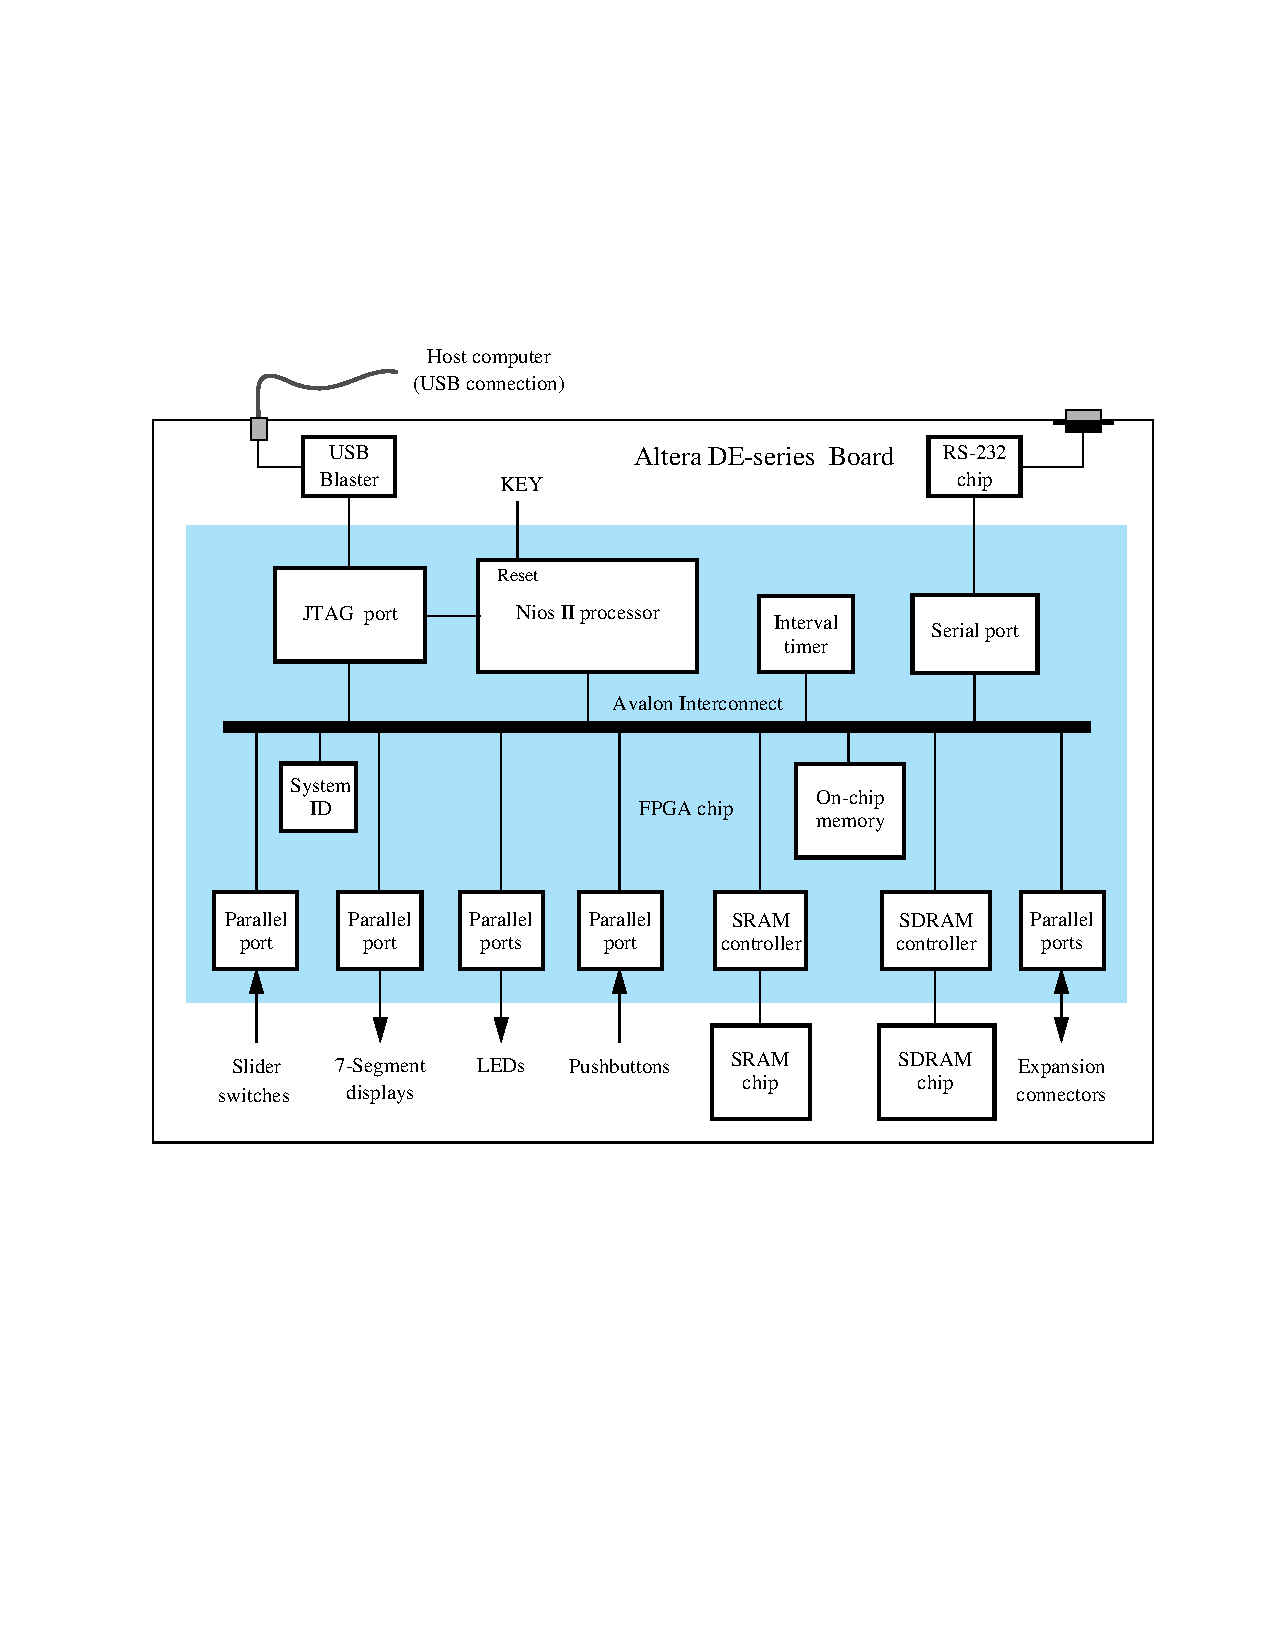
\includegraphics[width=6.5in]{figures/fig1.pdf}
   \end{center}
   \caption{Block diagram of an example Platform Designer system implemented on an FPGA board.}
	\label{fig:1}
\end{figure}

Each component in the system, referred to as a {\it Platform Designer component}, adheres to at least 
one of the Avalon\textsuperscript{\textregistered} Interfaces supported by Platform Designer.  With the interface defined for the 
component, Platform Designer is able to construct an interconnect structure, called the Avalon Interconnect,
which enables components to exchange data. The Platform Designer tool can generate a system based on the 
selected set of components and user parameters. The generated system contains Verilog or 
VHDL code for each component and the interconnect structure, allowing it to be synthesized, 
placed and routed for an FPGA device.

In this tutorial we explain what we mean by a Platform Designer component, describe the Avalon Interfaces 
in more detail, and show how to create a custom component that can be included in the Platform Designer 
list of available components.

\section{What is a Platform Designer Component?}

A Platform Designer component is a hardware subcircuit that is available as a library component for use
in the Platform Designer tool.  Typically, the contains two parts: the internal hardware 
modules, and the external Avalon Interfaces.  The internal modules are the circuits that 
implement the desired functionality of the Platform Designer component, while the Avalon Interfaces are 
used by the component to communicate with hardware modules that are external to the component.

There are many types of Avalon Interfaces; the most commonly used types are: 
\begin {itemize}
\item Avalon Clock Interface -- an interface that drives or receives clocks
\item Avalon Reset Interface -- an interface that provides reset capability
\item Avalon Memory-Mapped Interface (Avalon MM) -- an address-based read/write interface 
which is typical of master-slave connections
\item Avalon Streaming Interface (Avalon-ST) -- an interface that supports unidirectional 
flow of data
\item Avalon Conduit Interface -- an interface that accommodates individual signals or groups 
of signals that do not fit into any of the other Avalon Interface types. You can export 
the conduit signals to make connections external to the Platform Designer system.
\end{itemize}

A single component can use as many of these interface types as it requires. For example, 
a component might provide an Avalon-ST port for high-throughput data, in addition to an 
Avalon MM slave port for control.  All components must include the Avalon Clock and 
Reset Interfaces. Readers interested in more complete information about the Avalon Interfaces 
may consult the {\it Avalon Interface Specifications} document that can be found on 
the Intel website.

In this tutorial we will show how to develop a Platform Designer component that has an Avalon Memory-Mapped 
Interface and an Avalon Conduit Interface. The component is a 32-bit register that can be 
read or written as a memory-mapped slave device via the Avalon Interconnect and can be visible 
outside the system through a conduit signal.  The purpose of the conduit is to allow the 
register contents to be displayed on external components such as LEDs or 7-segment displays.
Thus, this register is similar to the output parallel ports shown in Figure~\ref{fig:1}.

If the register is to be used in a system such as the one depicted in Figure~\ref{fig:1}, 
then it should respond correctly to Nios~II instructions that store data into the register, 
or load data from it.  Let {\it D} be the 32-bit input data for the register, 
{\it byteenable} be the four-bit control input that indicates which byte(s) will be loaded 
with new data, and {\it Q} be the 32-bit output of the register.
In addition, it is necessary to provide clock and reset signals. 
Figures~\ref{fig:2} and~\ref{fig:4} show a suitable specification for the desired register, 
called {\it reg32}, in Verilog and VHDL, respectively.

Our register will be instantiated in a top-level module that provides the necessary
signals for connecting to an Avalon MM Interconnect. Let this module be 
called {\it reg32\_avalon\_interface}.  The Avalon MM Interface signals used in this
module are:
\begin{itemize}
\item {\it clock}
\item {\it resetn} -- active-low reset signal
\item {\it readdata} -- 32-bit data read from the register
\item {\it writedata} -- 32-bit data to be stored in the register
\item {\it read} -- active when a read (load) transaction is to be performed
\item {\it write} -- active when a write (store) transaction is to be performed
\item {\it byteenable} -- two-bit signal that identifies which bytes are being used
\item {\it chipselect} -- active when the register is being read or written
\end{itemize}

\noindent
The {\it reg32\_avalon\_interface} module also provides a 32-bit Avalon Conduit Interface 
signal called {\it Q\_export}.  Figures~\ref{fig:3} and~\ref{fig:5} show how this module 
can be specified in Verilog and VHDL code, respectively.

\begin{figure}[!h]
	\begin{lstlisting}[language=Verilog, xleftmargin=3cm]
module reg32 (clock, resetn, D, byteenable, Q);
    input clock, resetn;
    input [3:0] byteenable;
    input [31:0] D;
    output reg [31:0] Q;
		
    always@(posedge clock)
        if (!resetn)
            Q <= 32'b0;
        else
    begin
        // Enable writing to each byte separately
        if (byteenable[0]) Q[7:0] <= D[7:0];
            if (byteenable[1]) Q[15:8] <= D[15:8];
            if (byteenable[2]) Q[23:16] <= D[23:16];
            if (byteenable[3]) Q[31:24] <= D[31:24];
        end
endmodule
		\end{lstlisting}
	\caption{Verilog code for the 32-bit register.}
	\label{fig:2}
\end{figure}

 
\begin{figure}[!h]
	\begin{lstlisting}[language=Verilog, xleftmargin=1cm]
module reg32_avalon_interface (clock, resetn, writedata, readdata, write, read,
    byteenable, chipselect, Q_export);

    // signals for connecting to the Avalon fabric
    input clock, resetn, read, write, chipselect;
    input [3:0] byteenable;
    input [31:0] writedata;
    output [31:0] readdata;

    // signal for exporting register contents outside of the embedded system
    output [31:0] Q_export;

    wire [3:0] local_byteenable;
    wire [31:0] to_reg, from_reg;

    assign to_reg = writedata;

    assign local_byteenable = (chipselect & write) ? byteenable : 4'd0;

    reg32 U1 ( .clock(clock), .resetn(resetn), .D(to_reg), 
        .byteenable(local_byteenable), .Q(from_reg) );

    assign readdata = from_reg;
    assign Q_export = from_reg;
endmodule
		\end{lstlisting}
	\caption{Verilog code for the Avalon MM Interface.}
	\label{fig:3}
\end{figure}

\clearpage
\newpage
\begin{figure}[!h]
	\begin{lstlisting}[language=VHDL, xleftmargin=1.5cm]
LIBRARY ieee;
USE ieee.std_logic_1164.all;

ENTITY reg32 IS
    PORT ( clock, resetn : IN STD_LOGIC;
        D : IN STD_LOGIC_VECTOR(31 DOWNTO 0);
        byteenable : IN STD_LOGIC_VECTOR(3 DOWNTO 0);
        Q : OUT STD_LOGIC_VECTOR(31 DOWNTO 0) );
END reg32;

ARCHITECTURE Behavior OF reg32 IS
BEGIN
    PROCESS
    BEGIN
        WAIT UNTIL clock'EVENT AND clock = '1';
        IF resetn = '0'THEN
            Q <= "00000000000000000000000000000000";
        ELSE
            IF byteenable(0) = '1'THEN
                Q(7 DOWNTO 0) <= D(7 DOWNTO 0); END IF;
            IF byteenable(1) = '1'THEN
                Q(15 DOWNTO 8) <= D(15 DOWNTO 8); END IF;
            IF byteenable(2) = '1'THEN
                Q(23 DOWNTO 16) <= D(23 DOWNTO 16); END IF;
            IF byteenable(3) = '1'THEN
                Q(31 DOWNTO 24) <= D(31 DOWNTO 24); END IF;
        END IF;
    END PROCESS;
END Behavior;
		\end{lstlisting}
	\caption{VHDL code for the new register.}
	\label{fig:4}
\end{figure}

\clearpage
\newpage
\begin{figure}[!h]
	\begin{lstlisting}[language=VHDL, xleftmargin=1cm]
LIBRARY ieee;
USE ieee.std_logic_1164.all;

ENTITY reg32_avalon_interface IS
    PORT ( clock, resetn : IN STD_LOGIC;
        read, write, chipselect : IN STD_LOGIC;
        writedata : IN STD_LOGIC_VECTOR(31 DOWNTO 0);
        byteenable : IN STD_LOGIC_VECTOR(3 DOWNTO 0);
        readdata : OUT STD_LOGIC_VECTOR(31 DOWNTO 0);
        Q_export : OUT STD_LOGIC_VECTOR(31 DOWNTO 0) );
END reg32_avalon_interface;

ARCHITECTURE Structure OF reg32_avalon_interface IS
    SIGNAL local_byteenable : STD_LOGIC_VECTOR(3 DOWNTO 0);
    SIGNAL to_reg, from_reg : STD_LOGIC_VECTOR(31 DOWNTO 0);

    COMPONENT reg32
        PORT ( clock, resetn : IN STD_LOGIC;
            D : IN STD_LOGIC_VECTOR(31 DOWNTO 0);
            byteenable : IN STD_LOGIC_VECTOR(3 DOWNTO 0);
            Q : OUT STD_LOGIC_VECTOR(31 DOWNTO 0) );
    END COMPONENT;
BEGIN
    to_reg <= writedata;
    WITH (chipselect AND write) SELECT
        local_byteenable <= byteenable WHEN '1', "0000" WHEN OTHERS;
    reg_instance: reg32 PORT MAP (clock, resetn, to_reg, local_byteenable, from_reg);
    readdata <= from_reg;
    Q_export <= from_reg;
END Structure;
		\end{lstlisting}
	\caption{VHDL code for the memory-mapped new-register interface.}
	\label{fig:5}
\end{figure}

\section{Avalon\textsuperscript{\textregistered} Memory-Mapped Interface Details}

The Avalon Memory-Mapped Interface is a bus-like protocol that allows two components to 
exchange data.  One component implements a {\it master} interface that allows it to 
request and send data to {\it slave} components.  A slave component can only receive and 
process requests, either receiving data from the master, or providing the data 
requested by the master.

Each slave device includes one or more registers that can be accessed for read or write
transaction by a master device.  Figures~\ref{fig:6} and~\ref{fig:7} 
illustrate the signals that are used by master and slave interfaces.  
The direction of each signal is indicated by arrows beside it, with 
$\leftarrow$ indicating an output and $\rightarrow$ indicating an input to a device. 
All transactions are synchronized to the positive edge of the 
Avalon {\it clk} signal. At time $t_0$ in the figures, the master begins a read
transaction by placing a valid address on its {\it address} outputs and asserting 
its {\it read} control signal. The slave recognizes the request because its {\it chipselect}
input is asserted. It responds by placing valid data on its {\it readdata} outputs; the
master captures this data on its {\it readdata} inputs and the read transaction 
ends at time $t_1$. A second read transaction
is shown in the figure starting at time $t_2$. In this case, the slave device asserts the
{\it waitrequest} input of the master, which can be used to extend a read transaction by
any number of clock cycles. The slave device deasserts the {\it waitrequest} signal and
provides the requested data at time $t_3$, and the read transaction ends at time $t_4$. 

A write transaction is illustrated starting at time $t_5$ in Figures~\ref{fig:6} and~\ref{fig:7}.
The master places a valid address and data on its {\it address} and {\it datawrite} outputs,
and asserts the {\it write} control signal. The slave captures the data on its {\it datawrite}
inputs and the write transaction ends at time $t_6$.  
Although not shown in this example, a slave device can assert the 
{\it waitrequest} input of the master to extend a write transaction over multiple clock 
cycles if needed.

\begin{figure}[h!]
   \begin{center}
        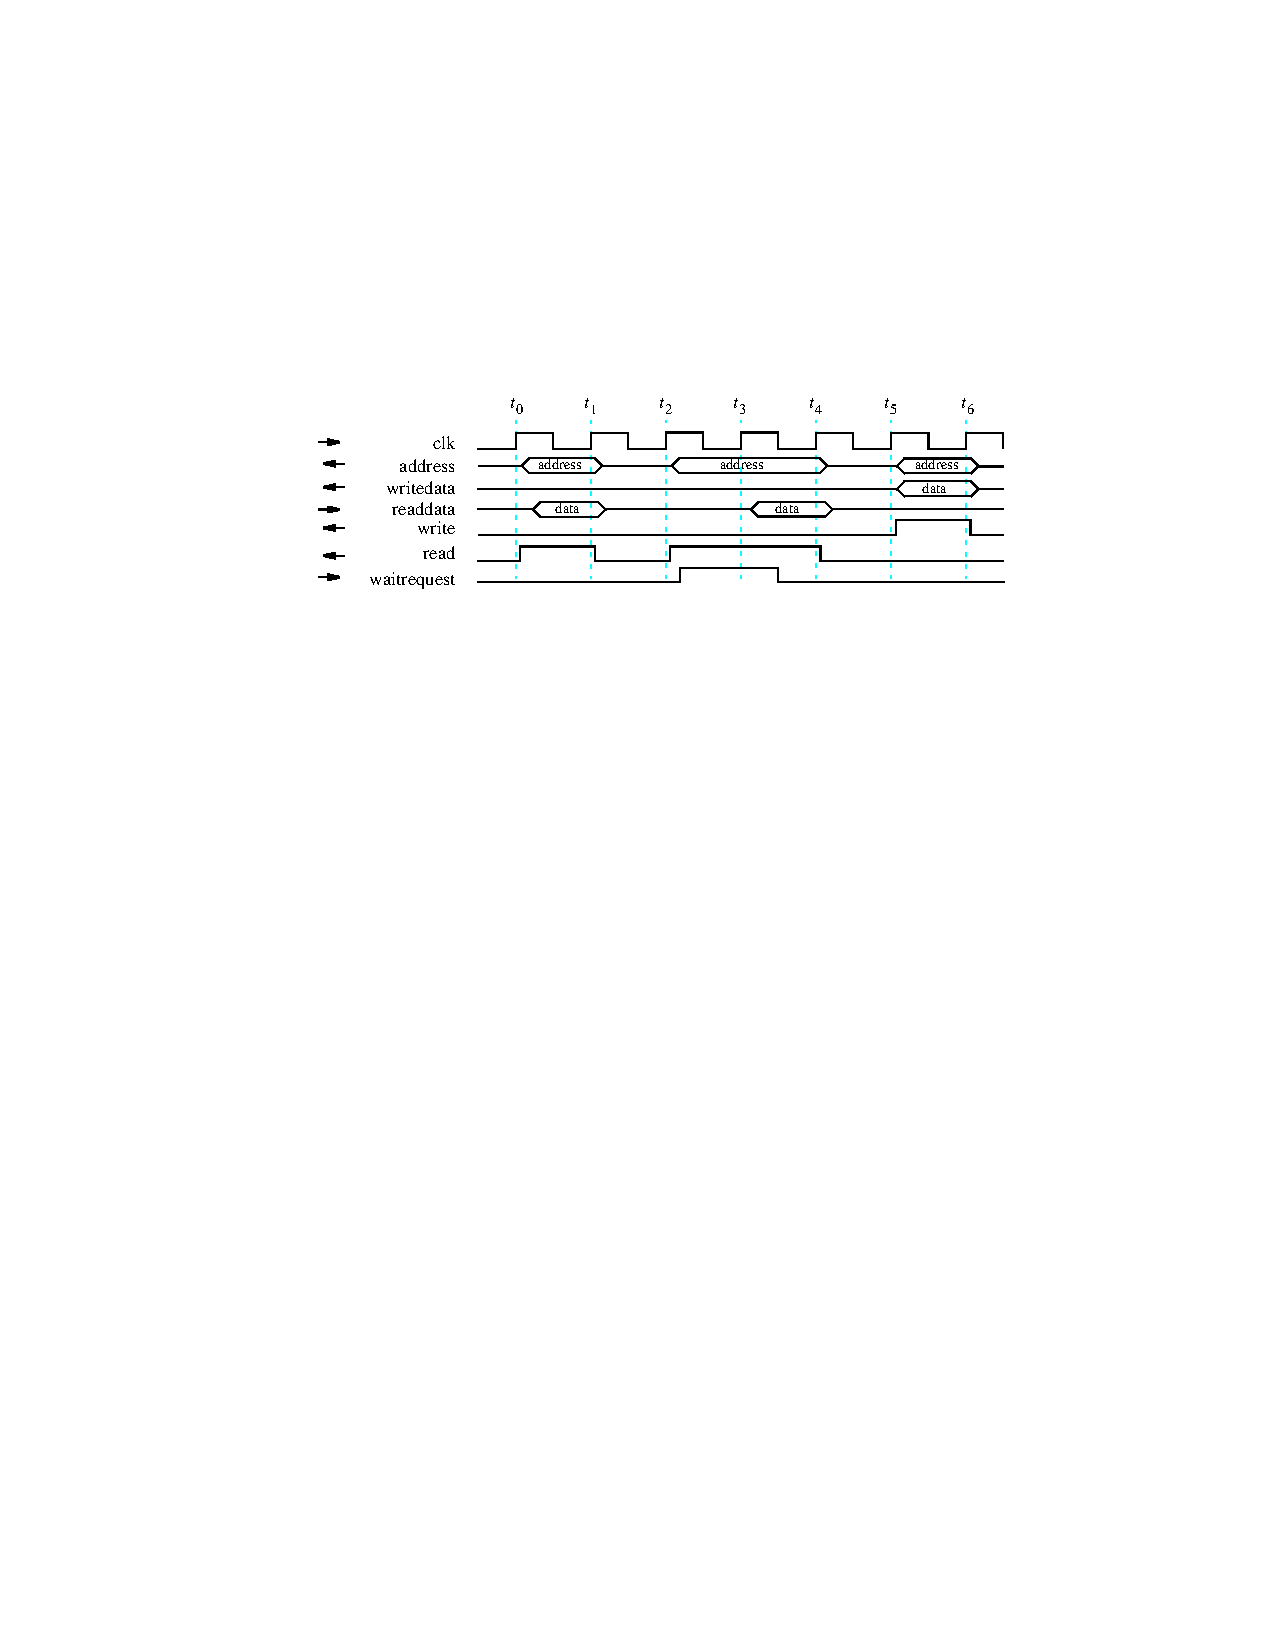
\includegraphics[scale=1.1]{figures/figure6.pdf}
   \end{center}
   \caption{Timing diagram for read/write transactions from the master's point of view.}
	\label{fig:6}
\end{figure}

\begin{figure}[h!]
   \begin{center}
        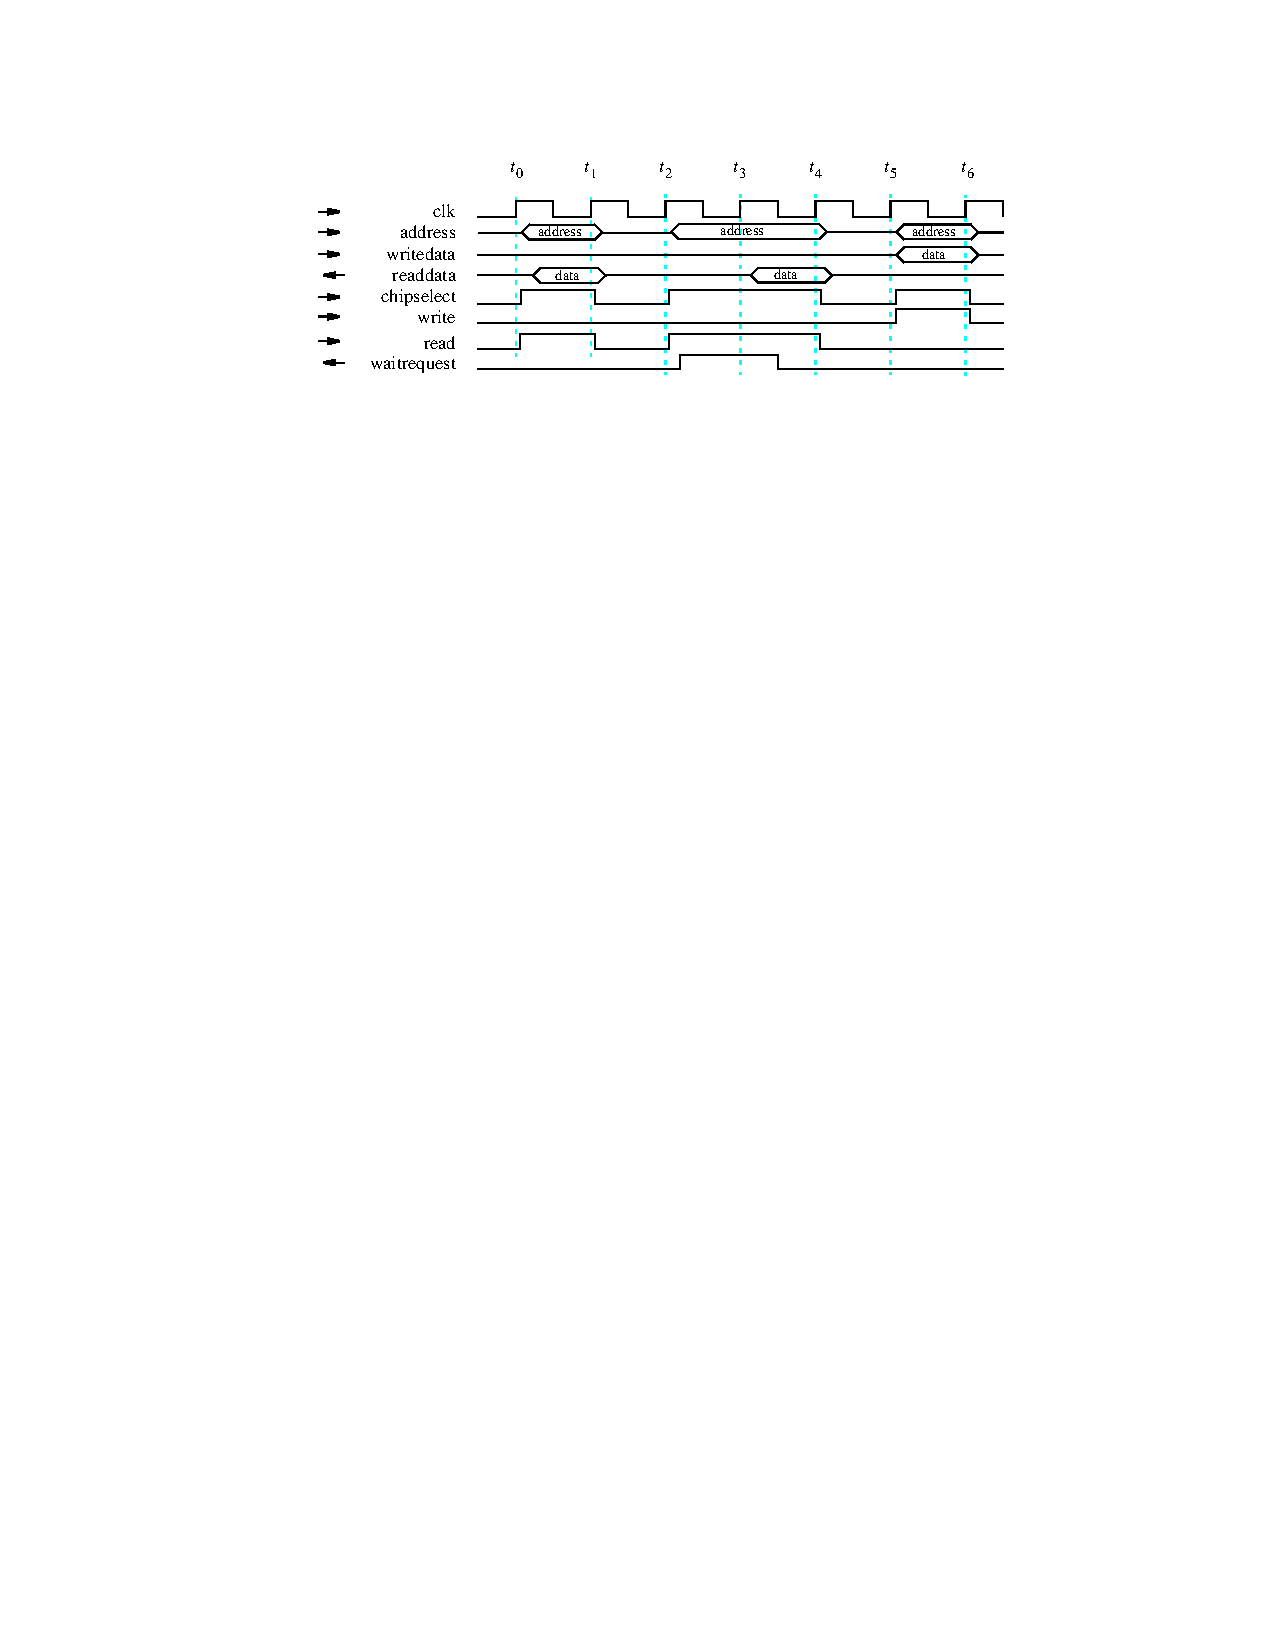
\includegraphics[scale=1.1]{figures/figure7.pdf}
   \end{center}
   \caption{Timing diagram for read/write transactions from the slave's point of view.}
	\label{fig:7}
\end{figure}

Addresses used by master devices are aligned to 32-bit word boundaries. For example, 
Figure~\ref{fig:8} illustrates four 32-bit addresses that could be used to select four
registers in a slave device. The address of the first register is {\sf 0x10000000}, the
address of the second register is {\sf 0x10000004}, and so on. In this example, the slave
would have a two-bit address input for selecting one of its four registers in any read or write
transaction. Since addresses are word-aligned, the lower two address bits from the master 
are not seen in the slave. The master provides a four-bit {\it byteenable} signal, which
is used by the slave to control a write transaction for individual bytes. For example, if the master
performs a write transaction to only the most-significant byte of the second register
in Figure~\ref{fig:8} then the master would write to address {\sf 0x10000007} by having its
{\it byteenable} output signal set to the value {\sf 0x1000} and its {\it address} output signal set to the value {\sf 0x10000004}.
The slave device would see its two-bit address input set to {\sf 0x01} and would use its {\it byteenable} inputs
to ensure that the write transaction is performed only for the selected byte of 
the second register. Although the {\it byteenable} signals are not shown in Figures~\ref{fig:6}
and~\ref{fig:7}, they have the same timing as the address signals.

The above examples show the basic transactions between a master and a slave. 
More advanced transactions can be performed, the procedure for which is described in 
the {\it Avalon Interconnect Specifications} document.

\begin{figure}[h!]
   \begin{center}
        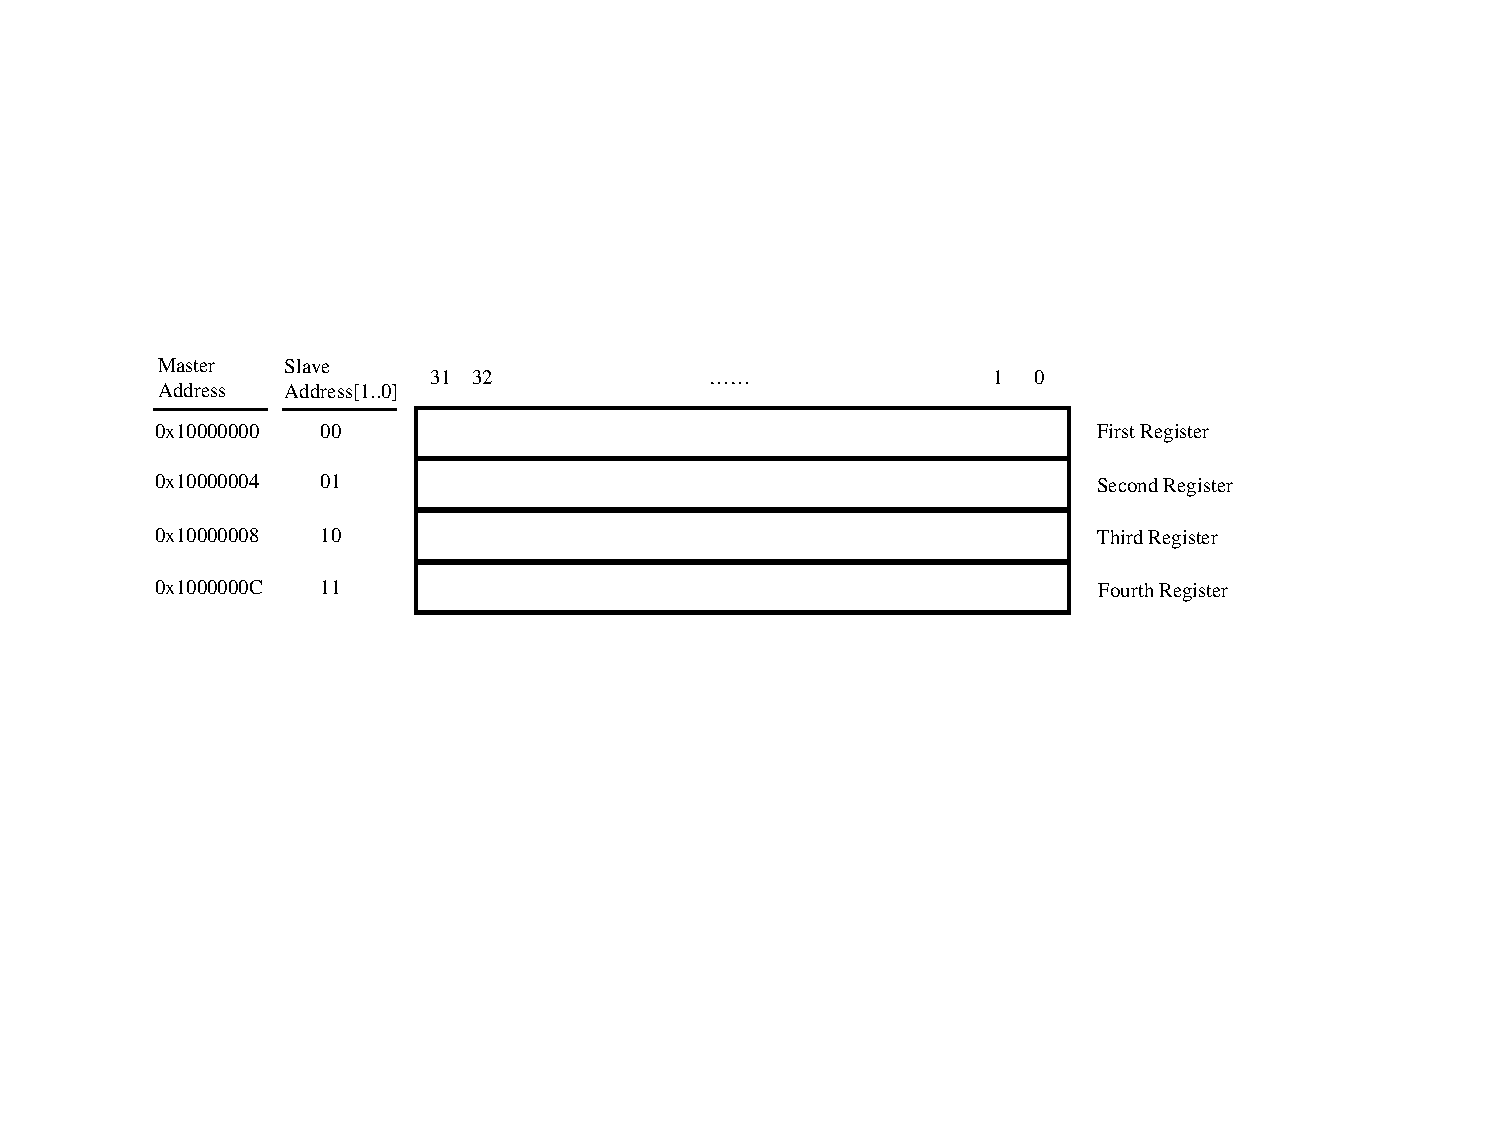
\includegraphics[scale=0.85]{figures/figure8.pdf}
   \end{center}
   \caption{Example for registers in an Avalon MM Interface.}
	\label{fig:8}
\end{figure}

\newpage
\section{Adding a New Component to the Platform Designer IP Catalog}

In this section we show how to create a new Platform Designer component for our 32-bit register defined
in Figures~\ref{fig:2} to \ref{fig:4}. As a first step, start the Quartus Prime software and
make a new project for use with this tutorial. Name the project {\it component\_tutorial}, and
choose the settings that are needed for your DE-series board, including the specific FPGA
chip.

Next, using your preferred HDL language (Verilog or VHDL), create a new design file {\sf (File $>$ New...
$>$ Design Files)} and add the Verilog code from Figure~\ref{fig:2}, or the VHDL code from Figure~\ref{fig:4}, and name the file {\it reg32.v (or .vhd)}. Add this file to your current project {\sf(Project $>$ Add Current File to Project)}. Create another file and add the Verilog code from Figure~\ref{fig:3} or the VHDL code from Figure~\ref{fig:5}, name the file {\it reg32\_avalon\_interface.v (or .vhd)}, and add this file to the current project.

Later, we will create a top-level HDL file for the {\it component\_tutorial} project, but
first we will use the Platform Designer tool to generate an embedded system.
Open the Platform Designer tool to get to the window depicted in Figure~\ref{fig:9}. The Platform Designer
tool automatically includes a clock component in the system, as shown in the figure. 

\begin{figure}[H]
   \begin{center}
        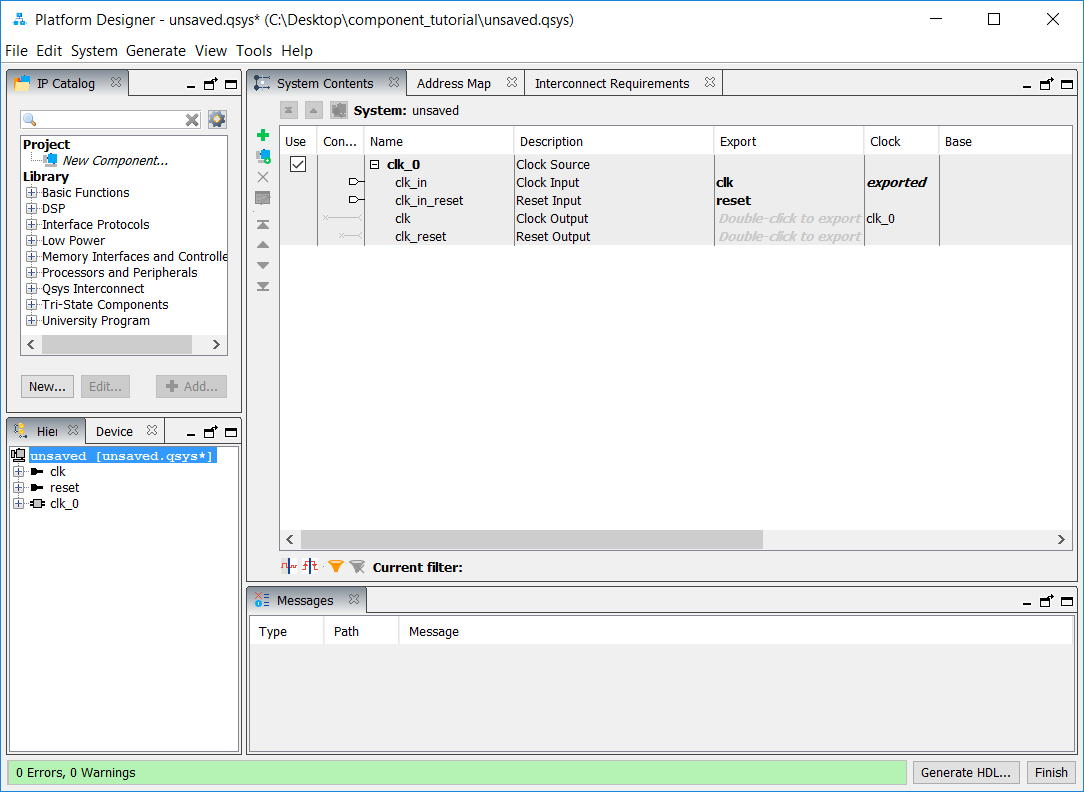
\includegraphics[width=0.9\textwidth]{figures/figure9.png}
   \end{center}
   \caption{Platform Designer window.}
	\label{fig:9}
\end{figure}

Before creating the new Platform Designer component for our 32-bit register, we will 
first instantiate some other components that will be needed in our system. In the {\sf IP Catalog} area of the Platform Designer window expand the
{\sf Processors and Peripherals $>$ Embedded Processors} item and add a {\sf Nios II Processor} to the system. In the Nios II
Processor dialog window that opens, select {\sf Nios II/e} as the type of processor. 
Next, in the {\sf IP Catalog}, expand the {\sf Basic Functions $>$ On-Chip Memory} item and add an {\sf On-Chip Memory (RAM or ROM) Intel FPGA IP} component.
Click {\sf Finish} to return to the main Platform Designer window. In the {\sf Connections} area of the Platform Designer
window, make the connections illustrated in Figure~\ref{fig:10} between 
the clock component, Nios II processor, and on-chip memory module. 

\begin{figure}[H]
   \begin{center}
        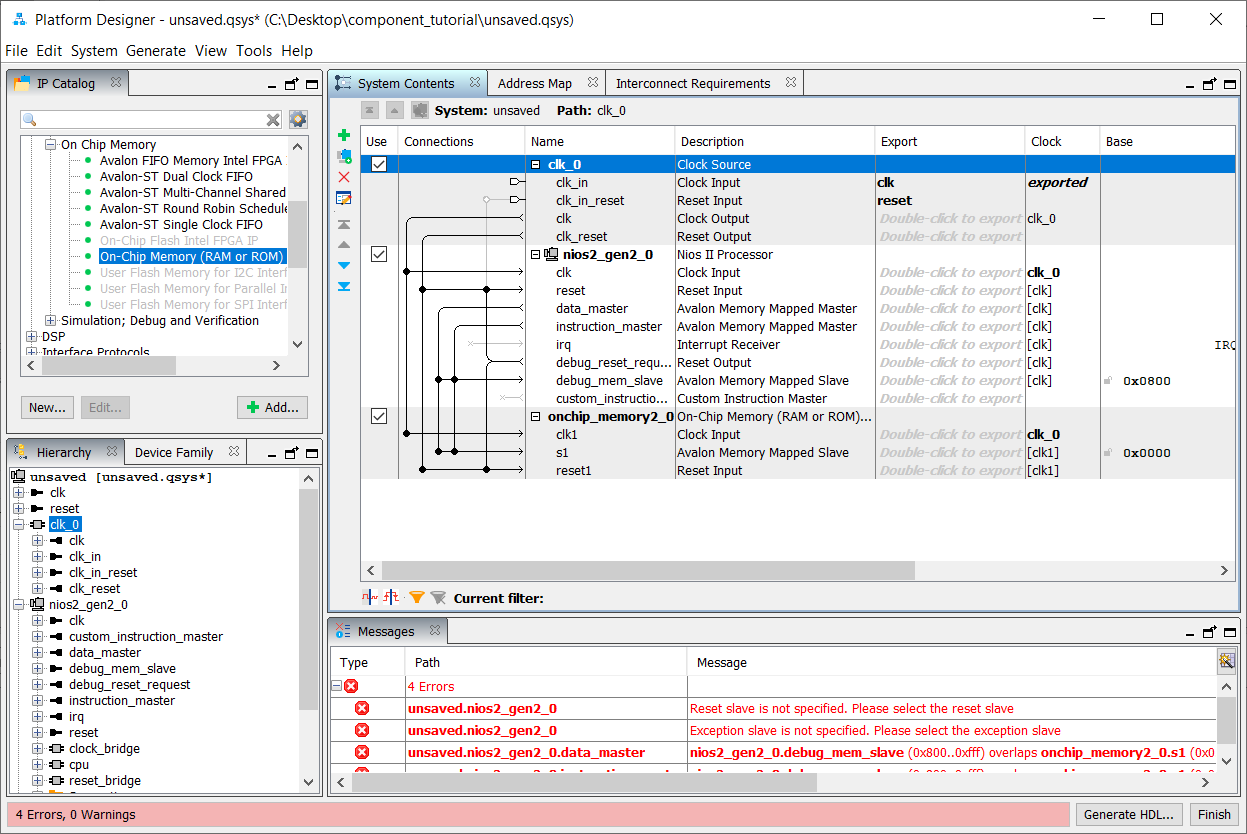
\includegraphics[width=0.9\textwidth]{figures/figure10.png}
   \end{center}
   \caption{Connections needed between components.}
	\label{fig:10}
\end{figure}

\newpage
Errors will be displayed in the Platform Designer {\sf Messages} window about the Reset and Exception
vectors memories that are needed for the Nios II Processor. To fix these errors, re-open the
Nios II processor component that has already been added to the system by right-clicking on it and selecting {\sf Edit}.
In the window shown in Figure~\ref{fig:11} use the provided drop-down menus to set both
the Reset vector memory and Exception vector memory to the on-chip memory component.
Click {\sf Finish} to return to the main Platform Designer window.

\begin{figure}[H]
   \begin{center}
        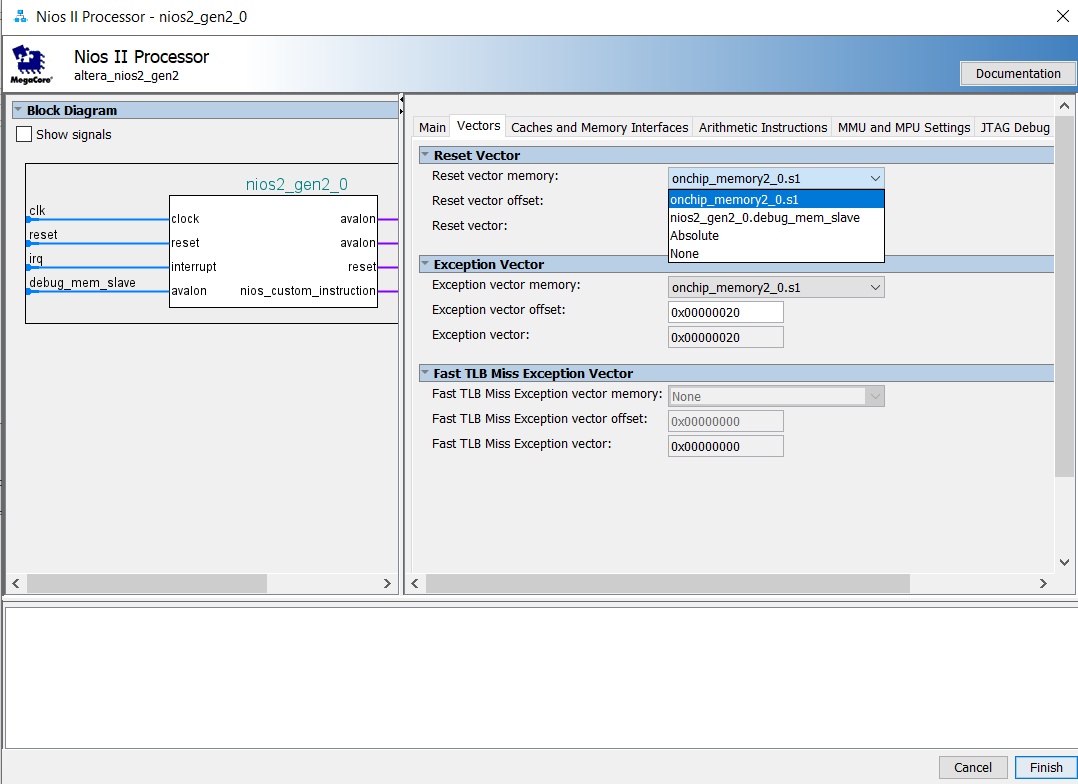
\includegraphics[width=0.8\textwidth]{figures/figure11.png}
   \end{center}
   \caption{Setting the reset and exception vector memories.}
	\label{fig:11}
\end{figure}

\newpage
The Platform Designer window may now show an error related to overlapping addresses assigned to the 
components in the system. To fix this error click on the {\sf System} menu in the Platform Designer window and 
then click on {\sf Assign Base Addresses}. The Platform Designer window should now appear as illustrated in
Figure~\ref{fig:12}. 

\begin{figure}[H]
   \begin{center}
        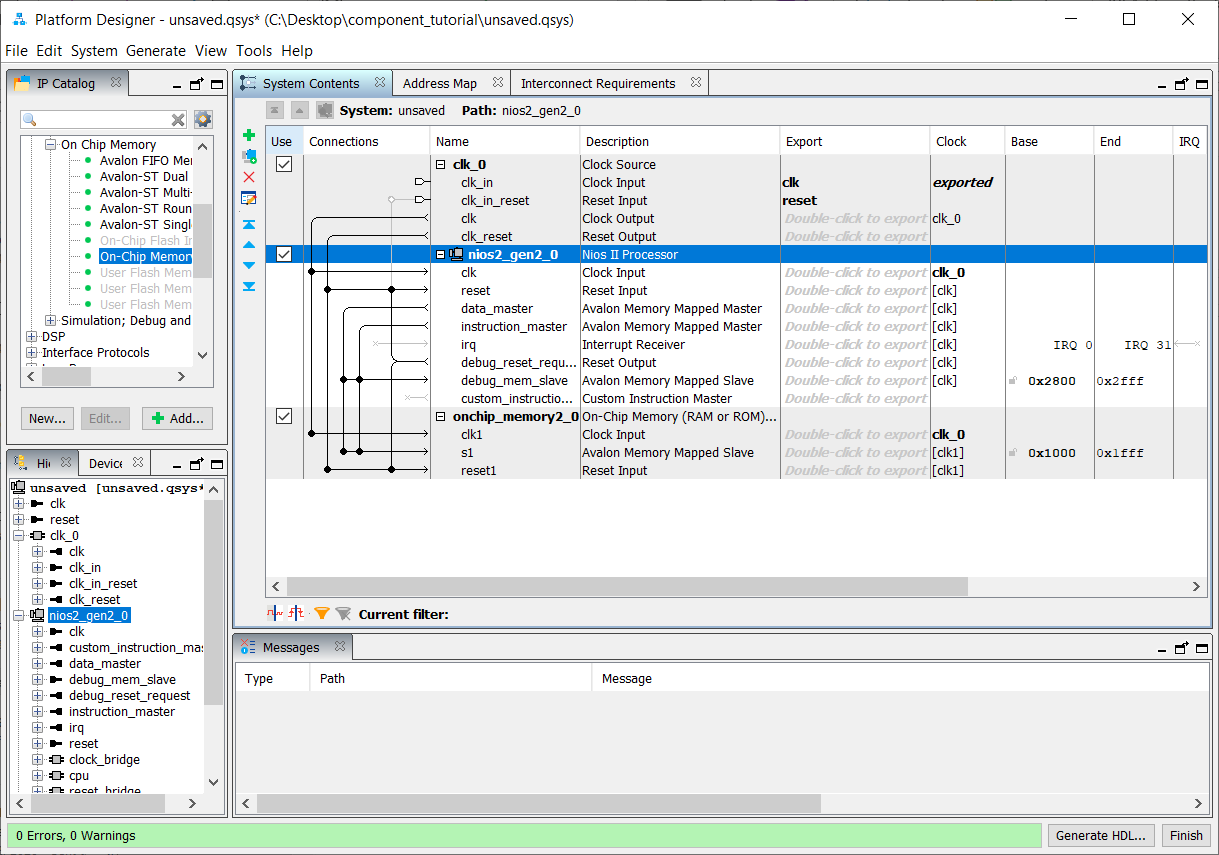
\includegraphics[width=0.9\textwidth]{figures/figure12.png}
   \end{center}
   \caption{The base Platform Designer system.}
	\label{fig:12}
	\end{figure}

\clearpage
\newpage
Now, we will create the new Platform Designer component for our 32-bit register, and make this
component available in the Platform Designer IP Catalog.
To create a new component, click the {\sf New...} button in the {\sf IP Catalog} area of
the Platform Designer window. The Component Editor tool, shown in Figure~\ref{fig:13}, 
will appear. It has four tabs. 

The first step in creating a component is to specify where in the 
IP Catalog our new component will appear. In the current tab, {\sf Component Type}, change the {\sf Name} to {\it reg32\_avalon\_interface}, the {\sf Display name} to {\it reg32\_component}, and
provide a name for the {\sf Group} setting, such as {\it My Own IP Cores}.

\begin{figure}[H]
   \begin{center}
        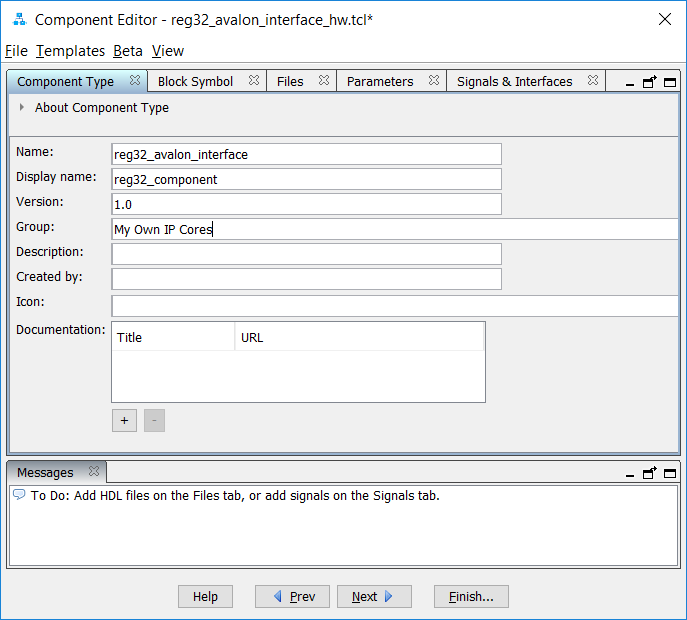
\includegraphics[scale=0.75]{figures/figure13.png}
   \end{center}
   \caption{Component Editor window.}
	\label{fig:13}
\end{figure}
\clearpage
\newpage
Next, we add the files that describe the component. Go to the {\sf Files} tab, depicted in
Figure~\ref{fig:14}, and then click on the {\sf Add File...} button under {\sf Synthesis Files} to browse and select the top-level 
file {\it reg32\_avalon\_interface.v}. Run the analysis of the top-level file by clicking on the {\sf Analyze Synthesis Files} button. Platform Designer analyzes this file to
determine the types of interfaces that are used by the component. Optionally, you can also
add the file {\it reg32.v} to the list of {\it Synthesis Files}. Then click the {\sf Copy from Synthesis Files} button under {\sf Verilog Simulation Files} to add the files for simulation. If the Component Editor finds any errors when analyzing the top-level file,
then they will need to be fixed and the code re-analyzed. Once no syntax errors are present, 
then the next step is to specify the types of interfaces that are used by the component.

\begin{figure}[H]
   \begin{center}
        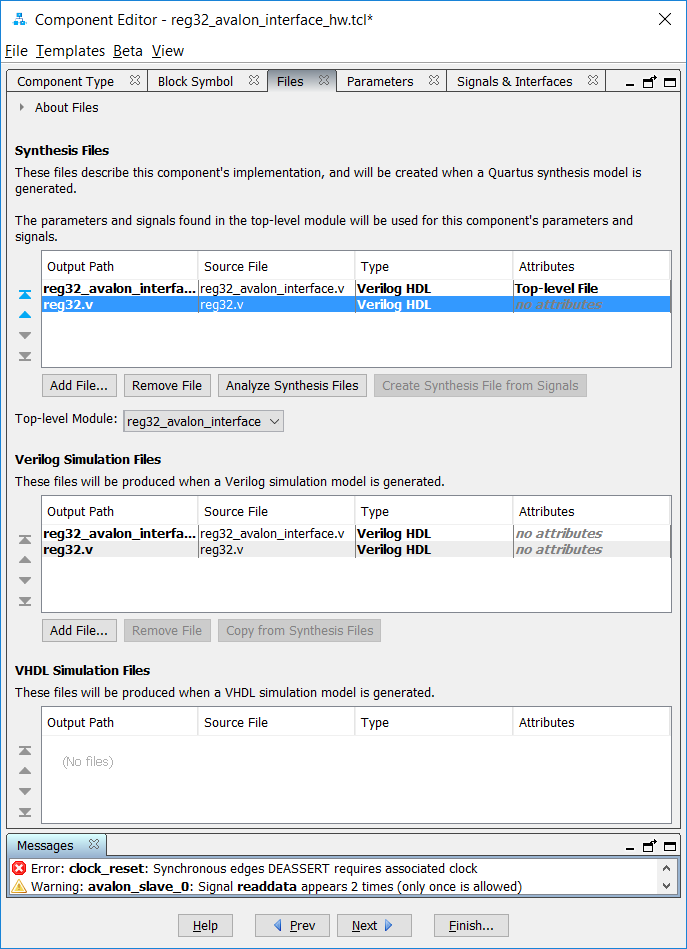
\includegraphics[scale=0.55]{figures/figure14.png}
   \end{center}
   \caption{Adding HDL files that define the new component.}
	\label{fig:14}
\end{figure}

\clearpage
\newpage
Click on the {\sf Signals \& Interfaces} tab to specify the meaning of each interface port in the 
top-level entity. This leads to the window in Figure~\ref{fig:15}. 

\begin{figure}[H]
   \begin{center}
        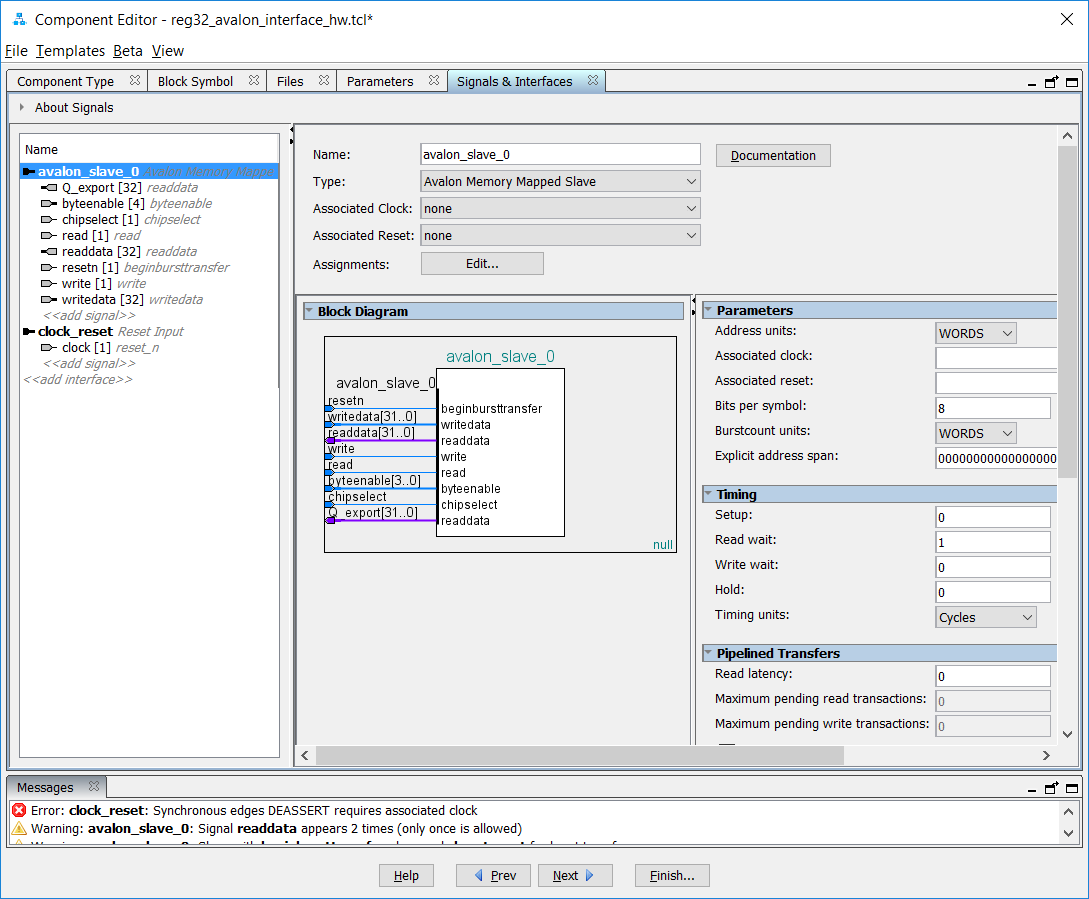
\includegraphics[scale=0.6]{figures/figure15.png}
   \end{center}
   \caption{Initial settings for component signals.}
	\label{fig:15}
\end{figure}

\clearpage
\newpage
To define correctly the meaning of each signal, it is necessary to specify the correct types of interface,
put the signals in the correct interface, and specify the signal type for each signal. For the {\it clock [1]} signal, 
select {\sf <{}<add interface>{}>} and select {\it Clock Input} as in Figure~\ref{fig:16}. Now drag and drop the signal {\it clock [1]} into {\it Clock Input} interface and change its {\it Signal Type} to {\it clk}, as shown in Figure~\ref{fig:17}.

\begin{figure}[H]
   \begin{center}
        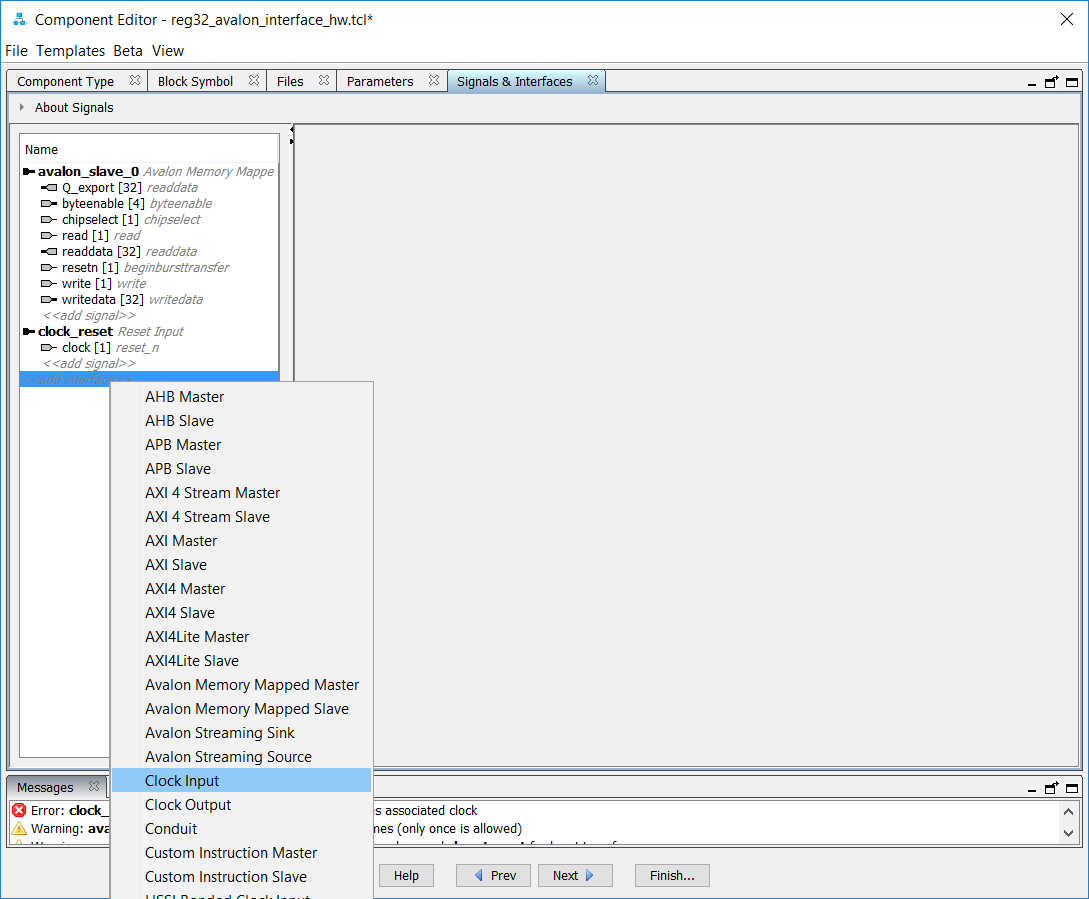
\includegraphics[scale=0.6]{figures/figure16.png}
   \end{center}
   \caption{Creating the {\it Clock Input} interface.}
	\label{fig:16}
\end{figure}

\clearpage

\begin{figure}[H]
   \begin{center}
        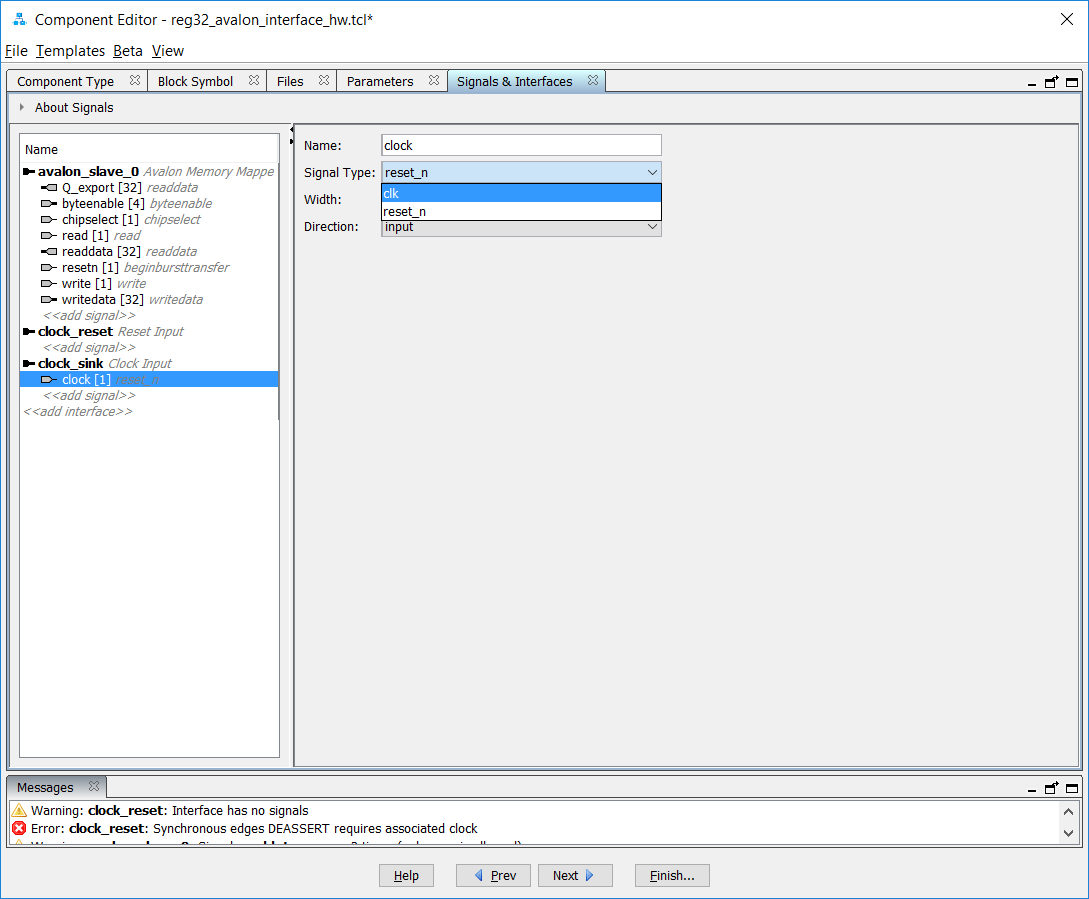
\includegraphics[scale=0.6]{figures/figure17.png}
   \end{center}
   \caption{Specifying the signal type for {\it clock}.}
	\label{fig:17}
\end{figure}

\clearpage
\newpage
For the {\it resetn [1]} signal, drag and drop it into the {\it Reset Input} interface
and change its signal type to {\it reset\_n}, as indicated in Figures~\ref{fig:18} 
and~\ref{fig:19}.

\begin{figure}[H]
   \begin{center}
        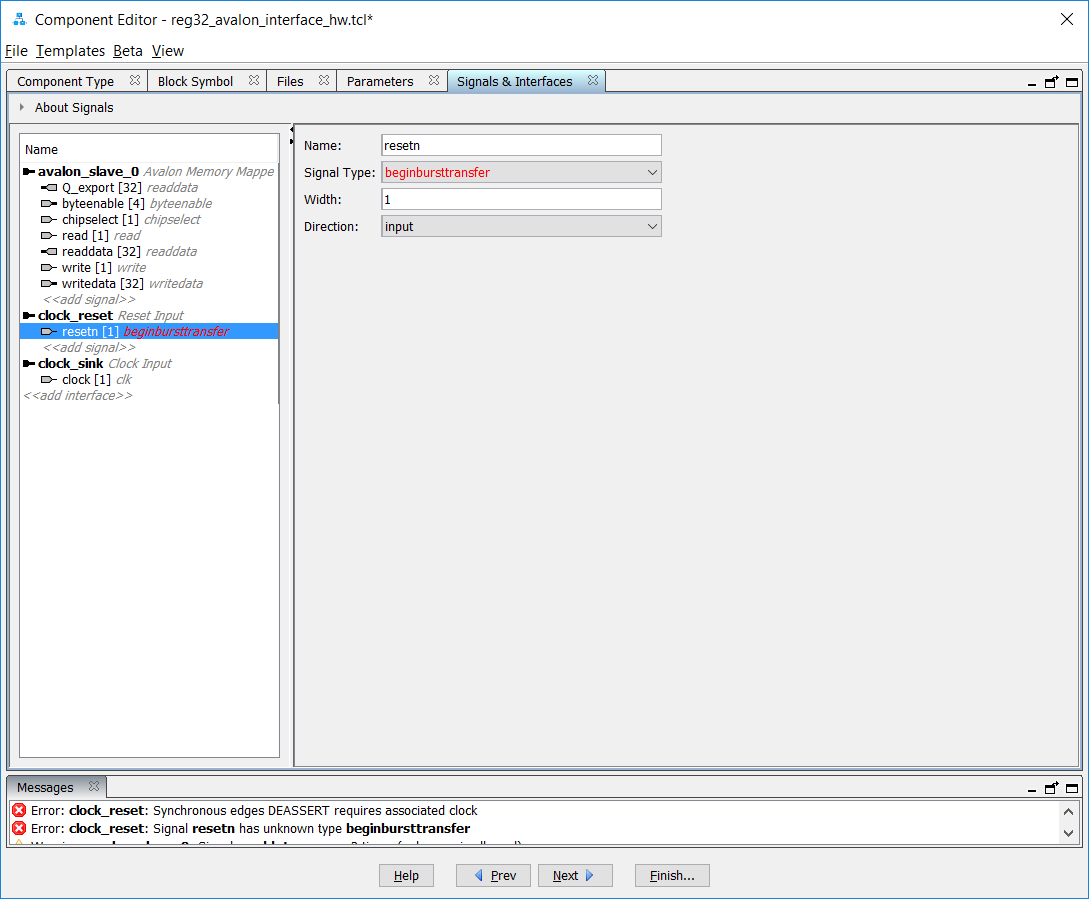
\includegraphics[scale=0.6]{figures/figure18.png}
   \end{center}
    \caption{Changing the interface for {\it resetn}.}
	\label{fig:18}
\end{figure}

\clearpage

\begin{figure}[H]
   \begin{center}
        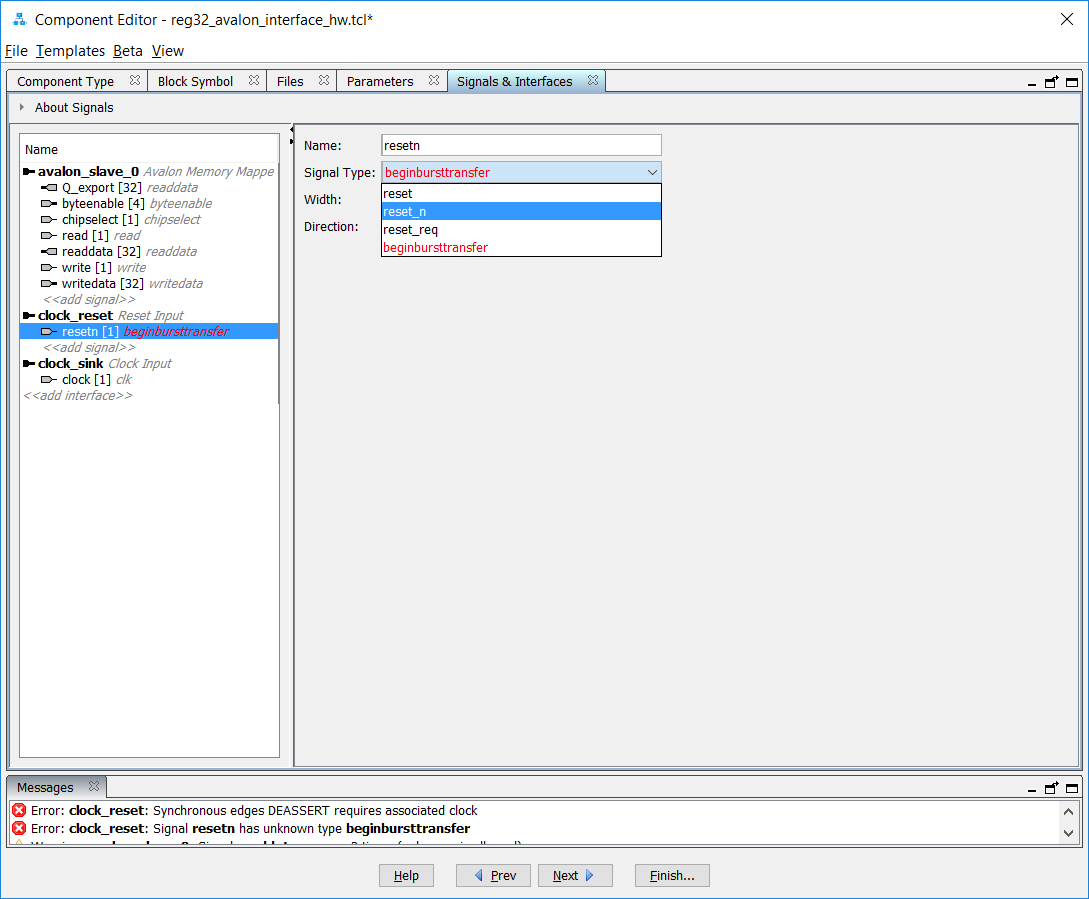
\includegraphics[scale=0.6]{figures/figure19.png}
   \end{center}
   \caption{Specifying the signal type for {\it resetn}.}
	\label{fig:19}
\end{figure}

\clearpage
\newpage
Finally, the {\it Q\_export} signal must be visible outside the 
Platform Designer-generated system; it requires a new interface which is not a part of the 
Avalon Memory-Mapped Interface.  Click on the {\sf <{}<add interface>{}>}, and specify its type as {\it Conduit}, as shown in Figure~\ref{fig:20}.
Drag and drop {\it Q\_export} into the newly created conduit interface. The {\it Signal Type} for a conduit signal does not matter, so {\it Q\_export} does not need to be edited. The rest of the signals shown in the Component Editor already have correct interface
types as their names are recognizable as specific Avalon signals.
The Component Editor window should now appear as shown in Figure~\ref{fig:21}.

\begin{figure}[H]
   \begin{center}
        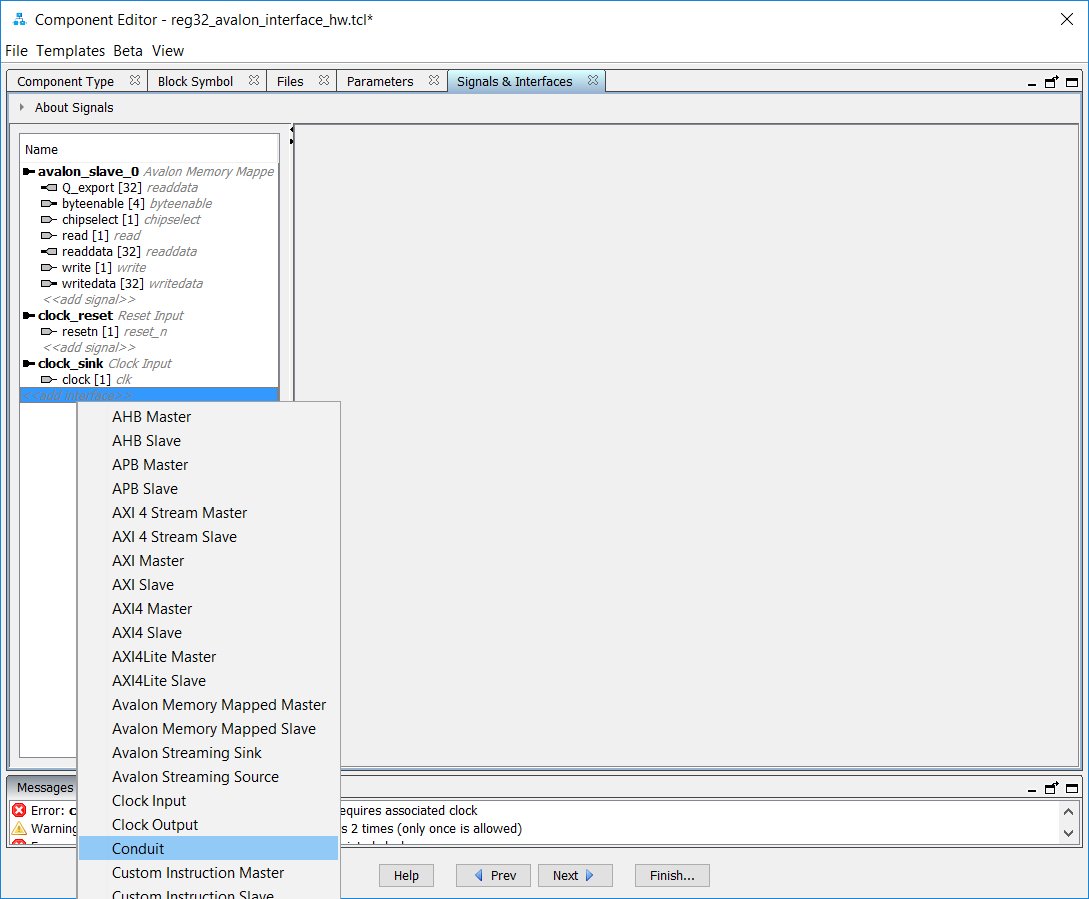
\includegraphics[scale=0.6]{figures/figure20.png}
   \end{center}
   \caption{Creating an external interface for {\it Q\_export}.}
	\label{fig:20}
\end{figure}

\clearpage

\begin{figure}[H]
   \begin{center}
        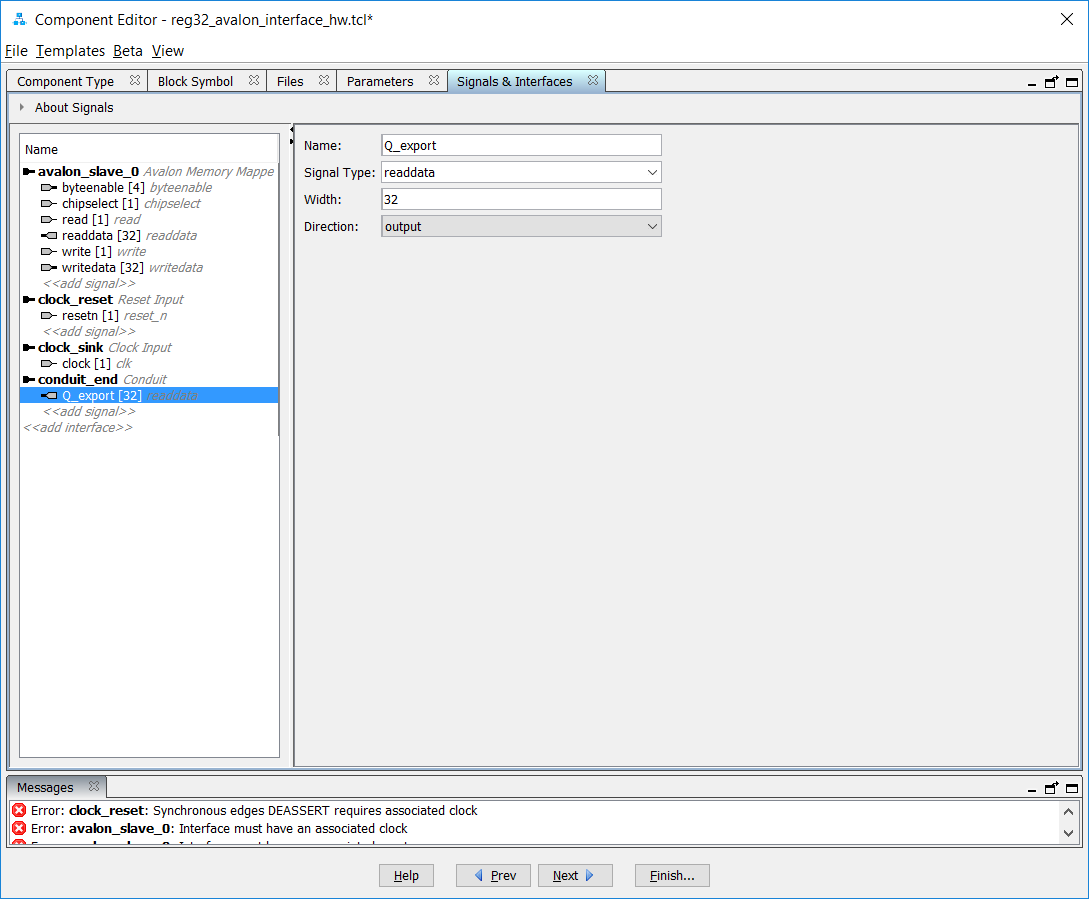
\includegraphics[scale=0.6]{figures/figure21.png}
   \end{center}
   \caption{Final settings for component signals.}
	\label{fig:21}
\end{figure}

\clearpage
\newpage
Note that there are still some error messages. The first error message states that the {\it avalon\_slave\_0} interface must have an 
Associated Clock and an Associated Reset.  Select {\it clock\_sink} as this clock 
and {\it clock\_reset} as the reset, as indicated in Figure~\ref{fig:22}.
Also note in Figure~\ref{fig:22} that under the {\sf Timing} heading we have changed the 
parameter called {\sf Read wait} for the {\it avalon\_slave\_0} interface from its 
default value, which was 1, to the value 0. This parameter represents the number of
Avalon clock signals that the component requires in order to respond to a read
request. Our register can respond immediately, so we do not need to use the default of 1 wait 
cycle.

\begin{figure}[H]
   \begin{center}
        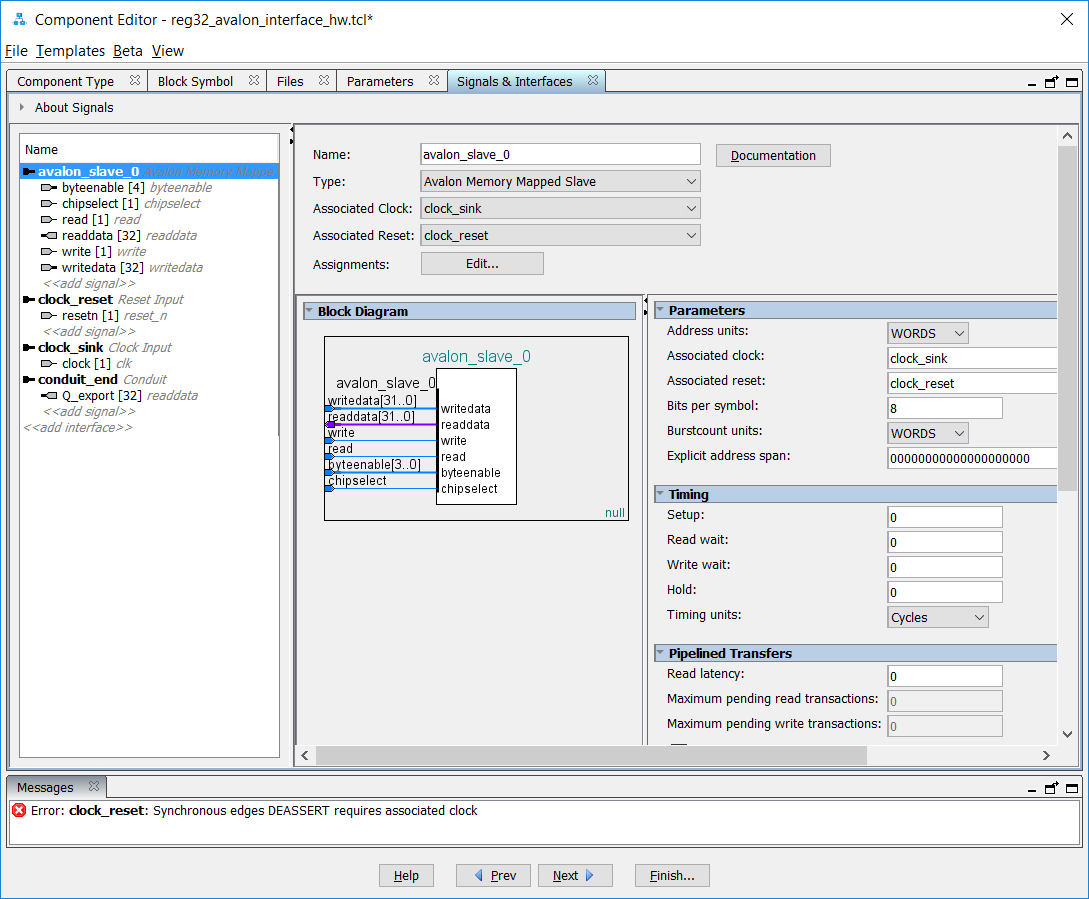
\includegraphics[scale=0.6]{figures/figure22.png}
   \end{center}
   \caption{Specifying the clock and reset associated with the Avalon Slave interface.}
	\label{fig:22}
\end{figure}

\clearpage
\newpage
The remaining error messages state that the {\it clock\_reset} interface must have an 
associated clock.  Set this clock to {\it clock\_sink}, as depicted in Figure~\ref{fig:23}.
Now, there should be no error messages left. Click {\sf Finish} to complete the creation of the Platform Designer component, and save 
the component when prompted to do so.
\begin{figure}[H]
   \begin{center}
        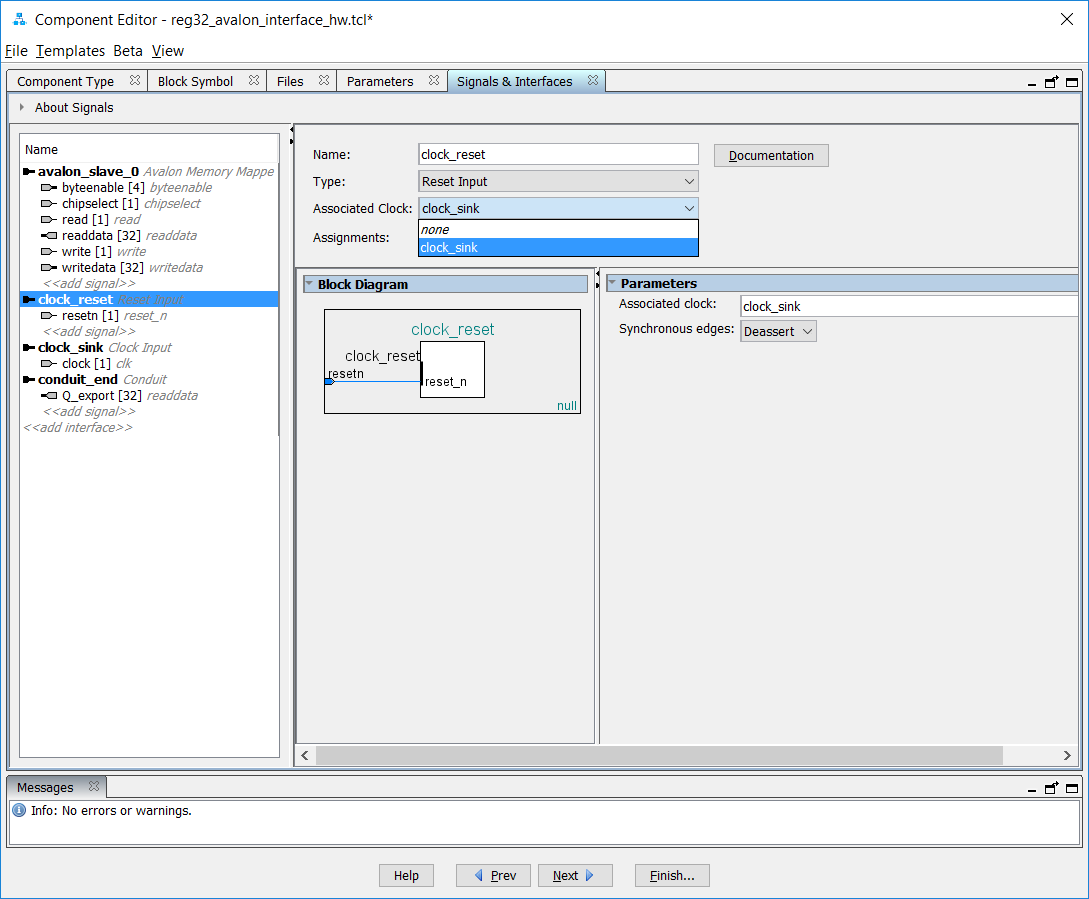
\includegraphics[scale=0.6]{figures/figure23.png}
   \end{center}
   \caption{Specifying the clock associated with the reset interface.}
	\label{fig:23}
\end{figure}

\newpage

\section{Instantiating the New Component}

In the Platform Designer IP Catalog, expand the newly-created item {\sf My Own IP Cores}. 
Add an instance of the {\it reg32\_component}, to open the window shown in
Figure~\ref{fig:24}. Click {\sf Finish} to return to the main Platform Designer window. 
\begin{figure}[h]
   \begin{center}
        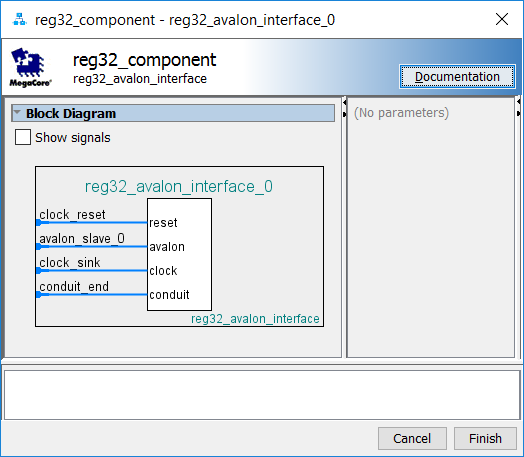
\includegraphics[scale=0.60]{figures/figure24.png}
   \end{center}
   \caption{Adding the {\it reg32\_component} to the base system.}
	\label{fig:24}
\end{figure}

Next, make the connections shown in Figure~\ref{fig:25} to attach the register component to the required
clock and reset signals, as well as to the data master port of the Nios II processor.
Finally, as indicated in the {\sf Export} column in Figure~\ref{fig:25}, click on 
{\sf Double-click to export} for the {\sf Conduit} and specify the name {\it to\_hex}.
Notice in the {\sf Base} address column in Figure~\ref{fig:25} that the assigned address
of the new register component is 00000000. This address can be directly edited by the
user, or it can be assigned automatically by using the {\sf Assign Base Addresses} command in
the {\sf System} menu. In this tutorial, we will leave the address as 00000000.

\begin{figure}[h]
   \begin{center}
        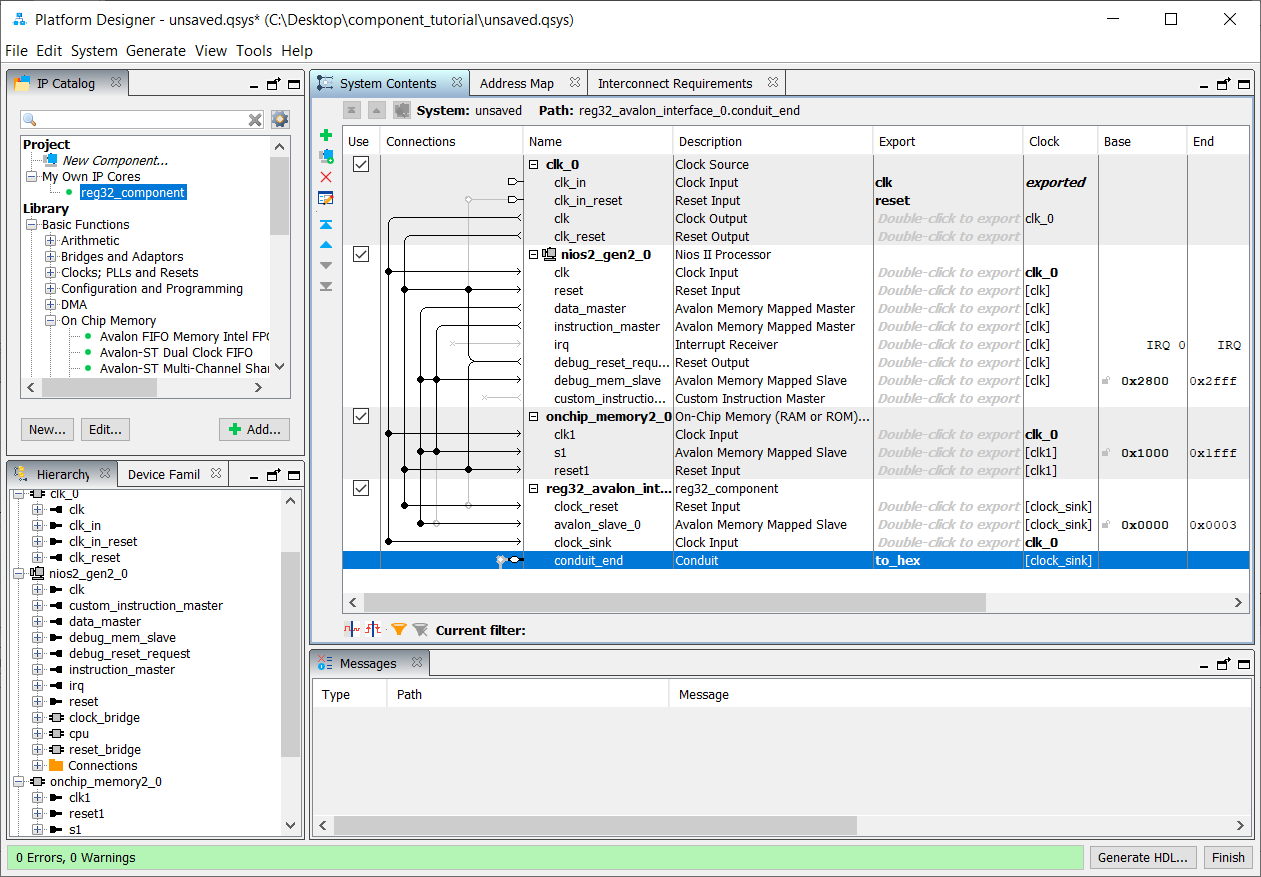
\includegraphics[width=0.85\textwidth]{figures/figure25.png}
   \end{center}
   \caption{Required connections for the new component.}
	\label{fig:25}
\end{figure}

Use the {\sf Save} command in the {\sf File} menu to save the defined Platform Designer system
using the name {\it embedded\_system}.
%Next, in the Platform Designer window click on the {\sf HDL Example} tab, shown in Figure~\ref{fig:26}. 
Next, in the Platform Designer window select {\sf Generate > Show Instantiation Template...}, the window in Figure~\ref{fig:26} will show up. 
This window gives an example of how the embedded system defined in the Platform Designer tool can 
be instantiated in HDL code. Note that the clock input of our embedded system is called 
{\it clk\_clk}, the reset input is called {\it resetn\_reset\_n}, and the conduit output is named
{\it to\_hex\_readdata}. 

\begin{figure}[H]
   \begin{center}
        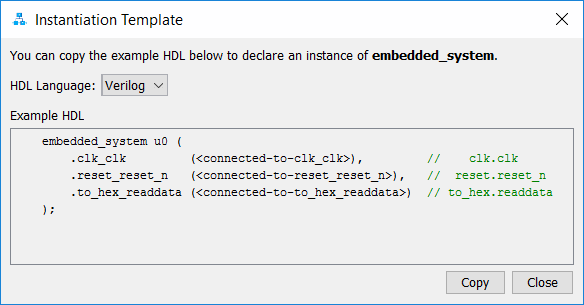
\includegraphics[width=0.6\textwidth]{figures/figure26.png}
   \end{center}
   \caption{The HDL Example tab.}
	\label{fig:26}
\end{figure}

\clearpage
\newpage
Finally, open the {\sf Generation} window in the Platform Designer tool, shown in Figure~\ref{fig:27} by selecting {\sf Generate $>$ Generate HDL},
and then click the {\sf Generate} button. This action causes the Platform Designer tool to generate HDL
code that specifies the contents of the embedded system, including all of the selected 
components and the Avalon interconnection fabric.

\begin{figure}[H]
   \begin{center}
        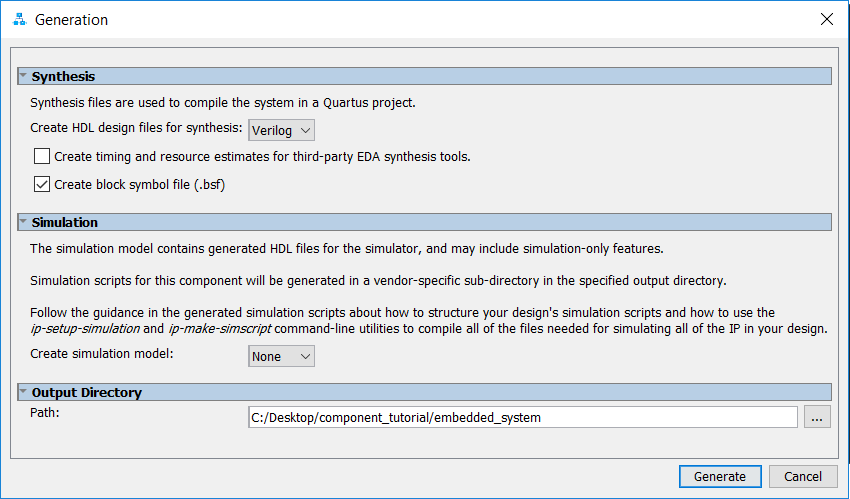
\includegraphics[width=0.9\textwidth]{figures/figure27.png}
   \end{center}
   \caption{The Generation tab.}
	\label{fig:27}
\end{figure}

\clearpage
\newpage
Close the Platform Designer tool to return to the main Quartus Prime window.
Next, select {\sf Project $>$ Add/Remove Files in Project...} from the main Quartus Prime window,
and then browse on the 
\includegraphics[scale=.6]{figures/icon1.png} button to open the window in
Figure~\ref{fig:28}. Browse to the folder called {\it embedded\_system/synthesis} and then select the file
named {\it embedded\_system.qip}. This file provides the information needed by the 
Quartus Prime software to locate the HDL code generated by the Platform Designer tool. In 
Figure~\ref{fig:28} click {\sf Open} to return to the {\sf Settings} window and then click
{\sf Add} to add the file to the project. Click {\sf OK} to return to the main Quartus Prime window.

\begin{figure}[H]
   \begin{center}
        
\includegraphics[scale=0.65]{figures/figure28.png}
   \end{center}
   \caption{Adding the .{\it qip} file to the Quartus Prime project.}
	\label{fig:28}
\end{figure}

\clearpage
\newpage
\section{Implementing the Embedded System in an FPGA Chip}
To implement the Platform Designer-generated embedded system in an FPGA chip, we need to 
create a top-level HDL module which instantiates the embedded system and has the appropriate 
input and output signals.  A suitable HDL module is given in
Figures~\ref{fig:29} and~\ref{fig:30}, in Verilog and VHDL. The module connects the 50 MHz
clock signal, {\it CLOCK}\_50, on the DE-series board to the clock input of the 
embedded system, and connects
{\it KEY}$_0$ to the reset input. The external conduit from the embedded system is
connected to the seven segment displays {\it HEX}0, $\ldots$, {\it HEX}3. The HDL code for
the 7-segment display code converter, called {\it hex7seg}, is provided in 
Appendix A, in Figures~\ref{fig:seg7v} and~\ref{fig:seg7vhdl}.

Store the code for the top-level module in a file called {\it component\_tutorial.v} 
(or {\it .vhd}), and store the code for the seven-segment code converter
in a file called {\it hex7seg.v} (or .{\it vhd}).
Include appropriate pin assignments in the Quartus~Prime project for the 
{\it CLOCK}\_50, {\it KEY}$_0$, and {\it HEX}0, $\ldots$, {\it HEX}3 signals on the 
DE-series board. If all the necessary pin assignments are not made, it may not be possible to connect to
the board (from the Quartus Prime software, or the \productNameMed{}). For instructions on adding
pin assignments, see the {\sf Quartus Introduction} tutorial.

Compile the project. After successful compilation, download the circuit onto the
DE-series board by using the Quartus~Prime Programmer tool. See the {\sf Quartus Introduction} tutorial
for instructions on downloading a circuit to a board.

\begin{figure}[!h]
	\begin{lstlisting}[language=Verilog]
module component_tutorial (CLOCK_50, KEY, HEX0, HEX1, HEX2, HEX3);
    input CLOCK_50;
    input [0:0] KEY;
    output [0:6] HEX0, HEX1, HEX2, HEX3;

    wire [15:0] to_HEX;

    embedded_system U0 (
        .clk_clk(CLOCK_50), .reset_reset_n(KEY[0]), .to_hex_readdata(to_HEX) );

    hex7seg h0(to_HEX[3:0], HEX0);
    hex7seg h1(to_HEX[7:4], HEX1);
    hex7seg h2(to_HEX[11:8], HEX2);
endmodule	
\end{lstlisting}
	\caption{Verilog code for the top-level module.}
	\label{fig:29}
\end{figure}

\clearpage
\newpage

\begin{figure}[!h]
	\begin{lstlisting}[language=VHDL]
LIBRARY ieee;
USE ieee.std_logic_1164.all;

ENTITY component_tutorial IS
    PORT ( CLOCK_50 : IN STD_LOGIC;
        KEY : IN STD_LOGIC_VECTOR(0 DOWNTO 0);
        HEX0 : OUT STD_LOGIC_VECTOR(0 TO 6);
        HEX1 : OUT STD_LOGIC_VECTOR(0 TO 6);
        HEX2 : OUT STD_LOGIC_VECTOR(0 TO 6);
        HEX3 : OUT STD_LOGIC_VECTOR(0 TO 6);
END component_tutorial;

ARCHITECTURE Structure OF component_tutorial IS
    SIGNAL to_HEX : STD_LOGIC_VECTOR(31 DOWNTO 0);
    COMPONENT embedded_system IS
        PORT ( clk_clk : IN STD_LOGIC;
            resetn_reset_n : IN STD_LOGIC;
            to_hex_readdata: OUT STD_LOGIC_VECTOR (31 DOWNTO 0) );
    END COMPONENT embedded_system;

    COMPONENT hex7seg IS
        PORT ( hex : IN STD_LOGIC_VECTOR(3 DOWNTO 0);
            display : OUT STD_LOGIC_VECTOR(0 TO 6) );
    END COMPONENT hex7seg;
BEGIN
    U0: embedded_system PORT MAP (
        clk_clk => CLOCK_50,
        resetn_reset_n => KEY(0),
        to_hex_readdata => to_HEX );
    h0: hex7seg PORT MAP (to_HEX(3 DOWNTO 0), HEX0);
    h1: hex7seg PORT MAP (to_HEX(7 DOWNTO 4), HEX1);
    h2: hex7seg PORT MAP (to_HEX(11 DOWNTO 8), HEX2);
    h3: hex7seg PORT MAP (to_HEX(15 DOWNTO 12), HEX3);
END Structure;	
\end{lstlisting}
	\caption{VHDL code for the top-level module.}
	\label{fig:30}
\end{figure}

\clearpage
\newpage
\section{Testing the Embedded System}
One way to test the circuit is to use the \productNameMed{}. Open the Monitor Program
and create a new project called {\it component\_tutorial} and select {\sf Nios II} as the architecture. In the {\sf New Project Wizard}, for
the {\sf Specify a system} screen choose {\sf <Custom System>}. As shown in the figure, under {\sf System details} browse to select the 
{\sf system description file} called {\it embedded\_system.sopcinfo}. Also, browse to select
the {\sf FPGA programming file} called {\it component\_tutorial.sof}, as illustrated in
Figure~\ref{fig:31}.  Select {\sf Not Required} for the {\sf Preloader}. For the screen titled {\sf Specify a program type} in the {\sf New Project
Wizard}, choose {\sf No Program}. On the next screen, specify the System Parameters according to your board, and then press {\sf Finish}. When prompted to download the system, as shown in Figure~\ref{fig:32}, press {\sf No} since we have already done so with the Quartus Prime Programmer. For a more detailed look at the FPGA Monitor Program, see the {\it Introduction to the Platform Designer Tool} tutorial on the University Program website.

\begin{figure}[H]
   \begin{center}
        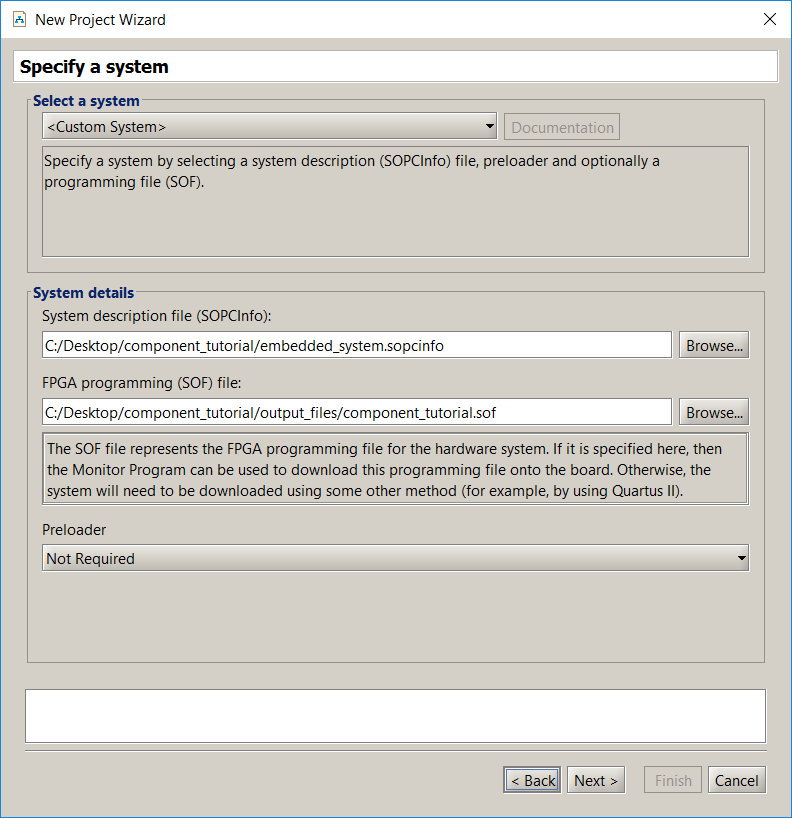
\includegraphics[scale=0.6]{figures/figure31.png}
   \end{center}
   \caption{Specifying the system description file and Quartus Prime programming file.}
	\label{fig:31}
\end{figure}

\clearpage

\begin{figure}[H]
   \begin{center}
        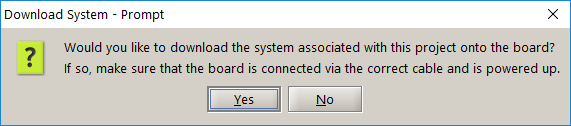
\includegraphics[scale=0.8]{figures/figure32.png}
   \end{center}
   \caption{Press {\sf No} to this prompt.}
	\label{fig:32}
\end{figure}

After successfully creating the Monitor Program project, click on the 
command {\sf Connect to System} in the {\sf Actions} menu. 
Open the {\sf Memory} tab in the Monitor Program, and click the setting {\sf Query 
Devices}, as indicated in Figure~\ref{fig:33}. Now, click the {\sf Refresh} button to 
see that the content of address {\sf 0x00000000}, which represents the 32-bit register 
component, has the value 00000000. 
%Since our register is a 16-bit component, it is useful to
%right-click in the {\sf Memory} tab, as shown in the figure, and make the 
%selection {\sf View as Half-word}.  
Edit the value stored in the register, as illustrated 
in Figure~\ref{fig:34}, and observe the changes on the seven-segment displays on the 
DE-series board.

\begin{figure}[H]
   \begin{center}
        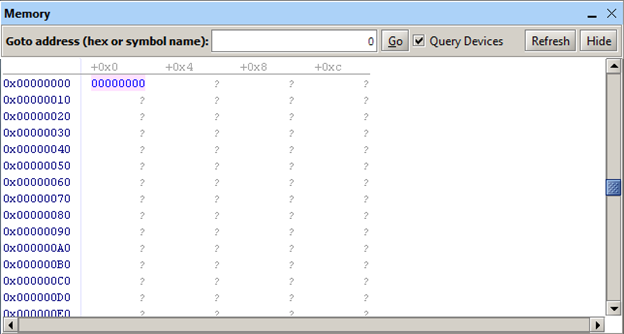
\includegraphics[scale=0.75]{figures/figure33.png}
   \end{center}
   \caption{Using the {\sf Memory} tab in the Momitor Program.}
	\label{fig:33}
\end{figure}

\clearpage

\begin{figure}[H]
   \begin{center}
        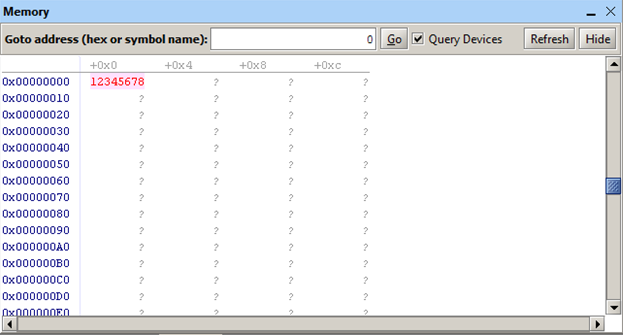
\includegraphics[scale=0.75]{figures/figure34.png}
   \end{center}
   \caption{Changing the value stored in the 32-bit register.}
	\label{fig:34}
\end{figure}

\section{Concluding Remarks}

In this tutorial we showed how to create a component for use in a system designed by using the 
Platform Designer tool.  Although the example is for a slave interface, the same procedure is used to 
create a master interface, with the only difference being in the type of an interface that is 
created for the component.

\clearpage
\newpage
\section{Appendix A}
The HDL code for the seven-segment code converter that is instantiated in
Figures~\ref{fig:29} and~\ref{fig:30} is shown in Figures~\ref{fig:seg7v} and~\ref{fig:seg7vhdl}.
\begin{figure}[!h]
	\centering
	\begin{lstlisting}[language=Verilog, xleftmargin=3.5cm]
module hex7seg (hex, display);
    input [3:0] hex;
    output [0:6] display;

    reg [0:6] display;
    /*
    *     - 0 -
    *  5 |     | 1
    *     - 6 -
    *  4 |     | 2
    *     - 3 -
    */
    always @ (hex)
        case (hex)
            4'h0: display = 7'b0000001;
            4'h1: display = 7'b1001111;
            4'h2: display = 7'b0010010;
            4'h3: display = 7'b0000110;
            4'h4: display = 7'b1001100;
            4'h5: display = 7'b0100100;
            4'h6: display = 7'b0100000;
            4'h7: display = 7'b0001111;
            4'h8: display = 7'b0000000;
            4'h9: display = 7'b0001100;
            4'hA: display = 7'b0001000;
            4'hb: display = 7'b1100000;
            4'hC: display = 7'b0110001;
            4'hd: display = 7'b1000010;
            4'hE: display = 7'b0110000;
            4'hF: display = 7'b0111000;
        endcase
endmodule
	\end{lstlisting}
	\caption{Verilog code for the seven-segment display code converter.}
	\label{fig:seg7v}
\end{figure}

\begin{figure}[!h]
	\begin{lstlisting}[language=VHDL, xleftmargin=3cm]
LIBRARY ieee;
USE ieee.std_logic_1164.all;

ENTITY hex7seg IS
    PORT ( hex : IN STD_LOGIC_VECTOR(3 DOWNTO 0);
        display : OUT STD_LOGIC_VECTOR(0 TO 6) );
END hex7seg;

ARCHITECTURE Behavior OF hex7seg IS
BEGIN
    --     - 0 -
    --  5 |     | 1
    --     - 6 -
    --  4 |     | 2
    --     - 3 -
    PROCESS (hex)
    BEGIN
        CASE hex IS
            WHEN "0000" => display <= "0000001";
            WHEN "0001" => display <= "1001111";
            WHEN "0010" => display <= "0010010";
            WHEN "0011" => display <= "0000110";
            WHEN "0100" => display <= "1001100";
            WHEN "0101" => display <= "0100100";
            WHEN "0110" => display <= "0100000";
            WHEN "0111" => display <= "0001111";
            WHEN "1000" => display <= "0000000";
            WHEN "1001" => display <= "0001100";
            WHEN "1010" => display <= "0001000";
            WHEN "1011" => display <= "1100000";
            WHEN "1100" => display <= "0110001";
            WHEN "1101" => display <= "1000010";
            WHEN "1110" => display <= "0110000";
            WHEN "1111" => display <= "0111000";
        END CASE;
    END PROCESS;
END Behavior;
	\end{lstlisting}
	\caption{VHDL code for the seven-segment display code converter.}
	\label{fig:seg7vhdl}
\end{figure}

% Copyright and Trademark

%\newcommand{\datePublished}{Mar 2022}

\newcommand{\versnum}{21.1} %version number quartus/AMP
\newcommand{\quartusname}{Quartus\textsuperscript{\textregistered} Prime}	
\newcommand{\textBar}{For \quartusname{} \versnum{}}
\newcommand{\thisyear}{2022 } %for copyright
\newcommand{\company}{FPGAcademy.org}
\newcommand{\longteamname}{FPGAcademy.org}
\newcommand{\teamname}{FPGAcademy}
\newcommand{\website}{FPGAcademy.org}

\newcommand{\productAcronym}{AMP}
\newcommand{\productNameShort}{Monitor Program}

\newcommand{\productNameMedTM}{Monitor Program}
\newcommand{\productNameMed}{Monitor Program}

%\newcommand{\headerLogoFilePath}[1]{#1/FPGAcademy.png}



%%%%%%%%%%%%%%%%%%%%%%%%%%%%%%%%%%%%%%%%
%%% FPGAcademy Copyright Information %%%
%%%%%%%%%%%%%%%%%%%%%%%%%%%%%%%%%%%%%%%%

%Always put the copyright on a new page (clear page), with some vertical space from top
\clearpage
\vspace{1in}

\noindent

Copyright {\copyright} FPGAcademy.org. All rights reserved. FPGAcademy and the FPGAcademy logo are trademarks of  FPGAcademy.org.  This document is being provided on an ``as-is'' basis and as an accommodation and therefore all warranties, representations or guarantees of any kind (whether express, implied or statutory) including, without limitation, warranties of merchantability, non-infringement, or fitness for a particular purpose, are specifically disclaimed.

%FPGAcademy assumes no responsibility or liability arising out of the application or use of any information,  product,  or  service  described  herein  except  as  expressly  agreed  to  in  writing  by  FPGAcademy.



**Other names and brands may be claimed as the property of others.




\end{document}
